\documentclass[10pt,landscape,oneside]{book}
\usepackage{caption}
\usepackage{etoolbox}
\usepackage[final]{grffile}
\usepackage{graphicx}
\usepackage{fancyvrb}
\usepackage[T1]{fontenc}
\usepackage{fancyhdr}
\usepackage{listings}
\usepackage{calc}
\graphicspath{{/home/mkg/Dropbox/images/}}
\pagestyle{headings}
\usepackage{lipsum}
\usepackage[hidelinks=true,linktoc=all]{hyperref}
\urlstyle{same}
\usepackage[all]{hypcap}\begin{document}
\frontmatter
\title{Selected Photographs}
\author{Michael Gogins \\ \texttt{michael.gogins@gmail.com}}
%\subtitle{Volume I}
%\dedication{This book is for Mick.}
.
\newpage
\noindent This book is copyright 2019 by Michael Gogins, all rights reserved. The contents of this book are licensed under the terms of the Creative Commons \href{https://creativecommons.org/licenses/by-nc-nd/4.0/legalcode}{\textbf{Attribution-NonCommercial-NoDerivatives 4.0 International} } license. In short, you may use, print, and copy this book or any of its contents for your own personal use, but you may not use this book or any of its contents as part of your own projects, or for commercial purposes.

If you wish to use this book or any of its contents for your own projects, or for commercial purposes, for example to re-publish or to exhibit in a gallery, please contact me directly.
\maketitle

\tableofcontents
\listoffigures

\mainmatter
\pagestyle{headings}

\chapter{Introduction}

This book contains my selection of 500 pictures from a lifetime of taking photographs. I have never been a professional, but I was and still am committed to the art of photography. These pictures were variously taken with 35 mm film cameras, a variety of digital cameras, and smartphones. They were taken in ny native state of Utah, the state of Washington, California, New York, other states, and various countries around the world. 

I am a ``street photographer`` open to abstraction. I shoot what catches my eye and I prize beauty. When I take pictures of people, I often prefer they don't notice. My reason for doing photography is to see more clearly what God has created.

I have tended to use the sharpest possible camera that is small enough to carry with me at all times. For some years now I have been using the Sony RX100 series. Increasingly, however, I am finding that my smartphone is a real camera.

As the file size of this book would become unmanageable thanks to the use of uncompressed images, it has been split into a number of volumes. Even so, the files are huge. However, they do enable the reader to zoom into the images in full detail or to extract them for printing at high resolution.

If I take more pictures that I think are good enough to be in this book, I will add them, and remove as many that are not quite good enough, to keep the total at 500 pictures.

\chapter{Photographs}

These images are all in natural color. They are all shot as far as possible without image manipulation; in a few cases, I have leveled horizons or removed spots. I shoot in JPEG rather than RAW. Selected metadata from the photographs is printed. If the photograph is a digital scan of a 35 mm slide, the creation date is the date of that scan. Captions are sporadic and cryptic, to say the least.

All pictures are included in the full resolution with which they were taken. Thus, you can zoom into any image to see more detail. Pictures copied out of this book will also be in full resolution.

I invite the reader to copy pictures out of this book for printing and viewing, but not for commercial use or re-publication. 




\KOMAoptions{pagesize}
\clearpage
\recalctypearea
\newpage
\noindent
Filename: None\\ 
Date taken: 2013:03:12 12:07:26\\ 
GPS longitude: None\\ 
GPS latitude: None\\ 
Make: None\\ 
Model: None\\ 
Focal length (35mm eq): None\\ 
Exposure: None\\ 
F stop: None\\ 
ISO: None\\ 
Width: None\\ 
Height: None\\ 

\clearpage
\recalctypearea
\newpage
\noindent
\begin{figure}
    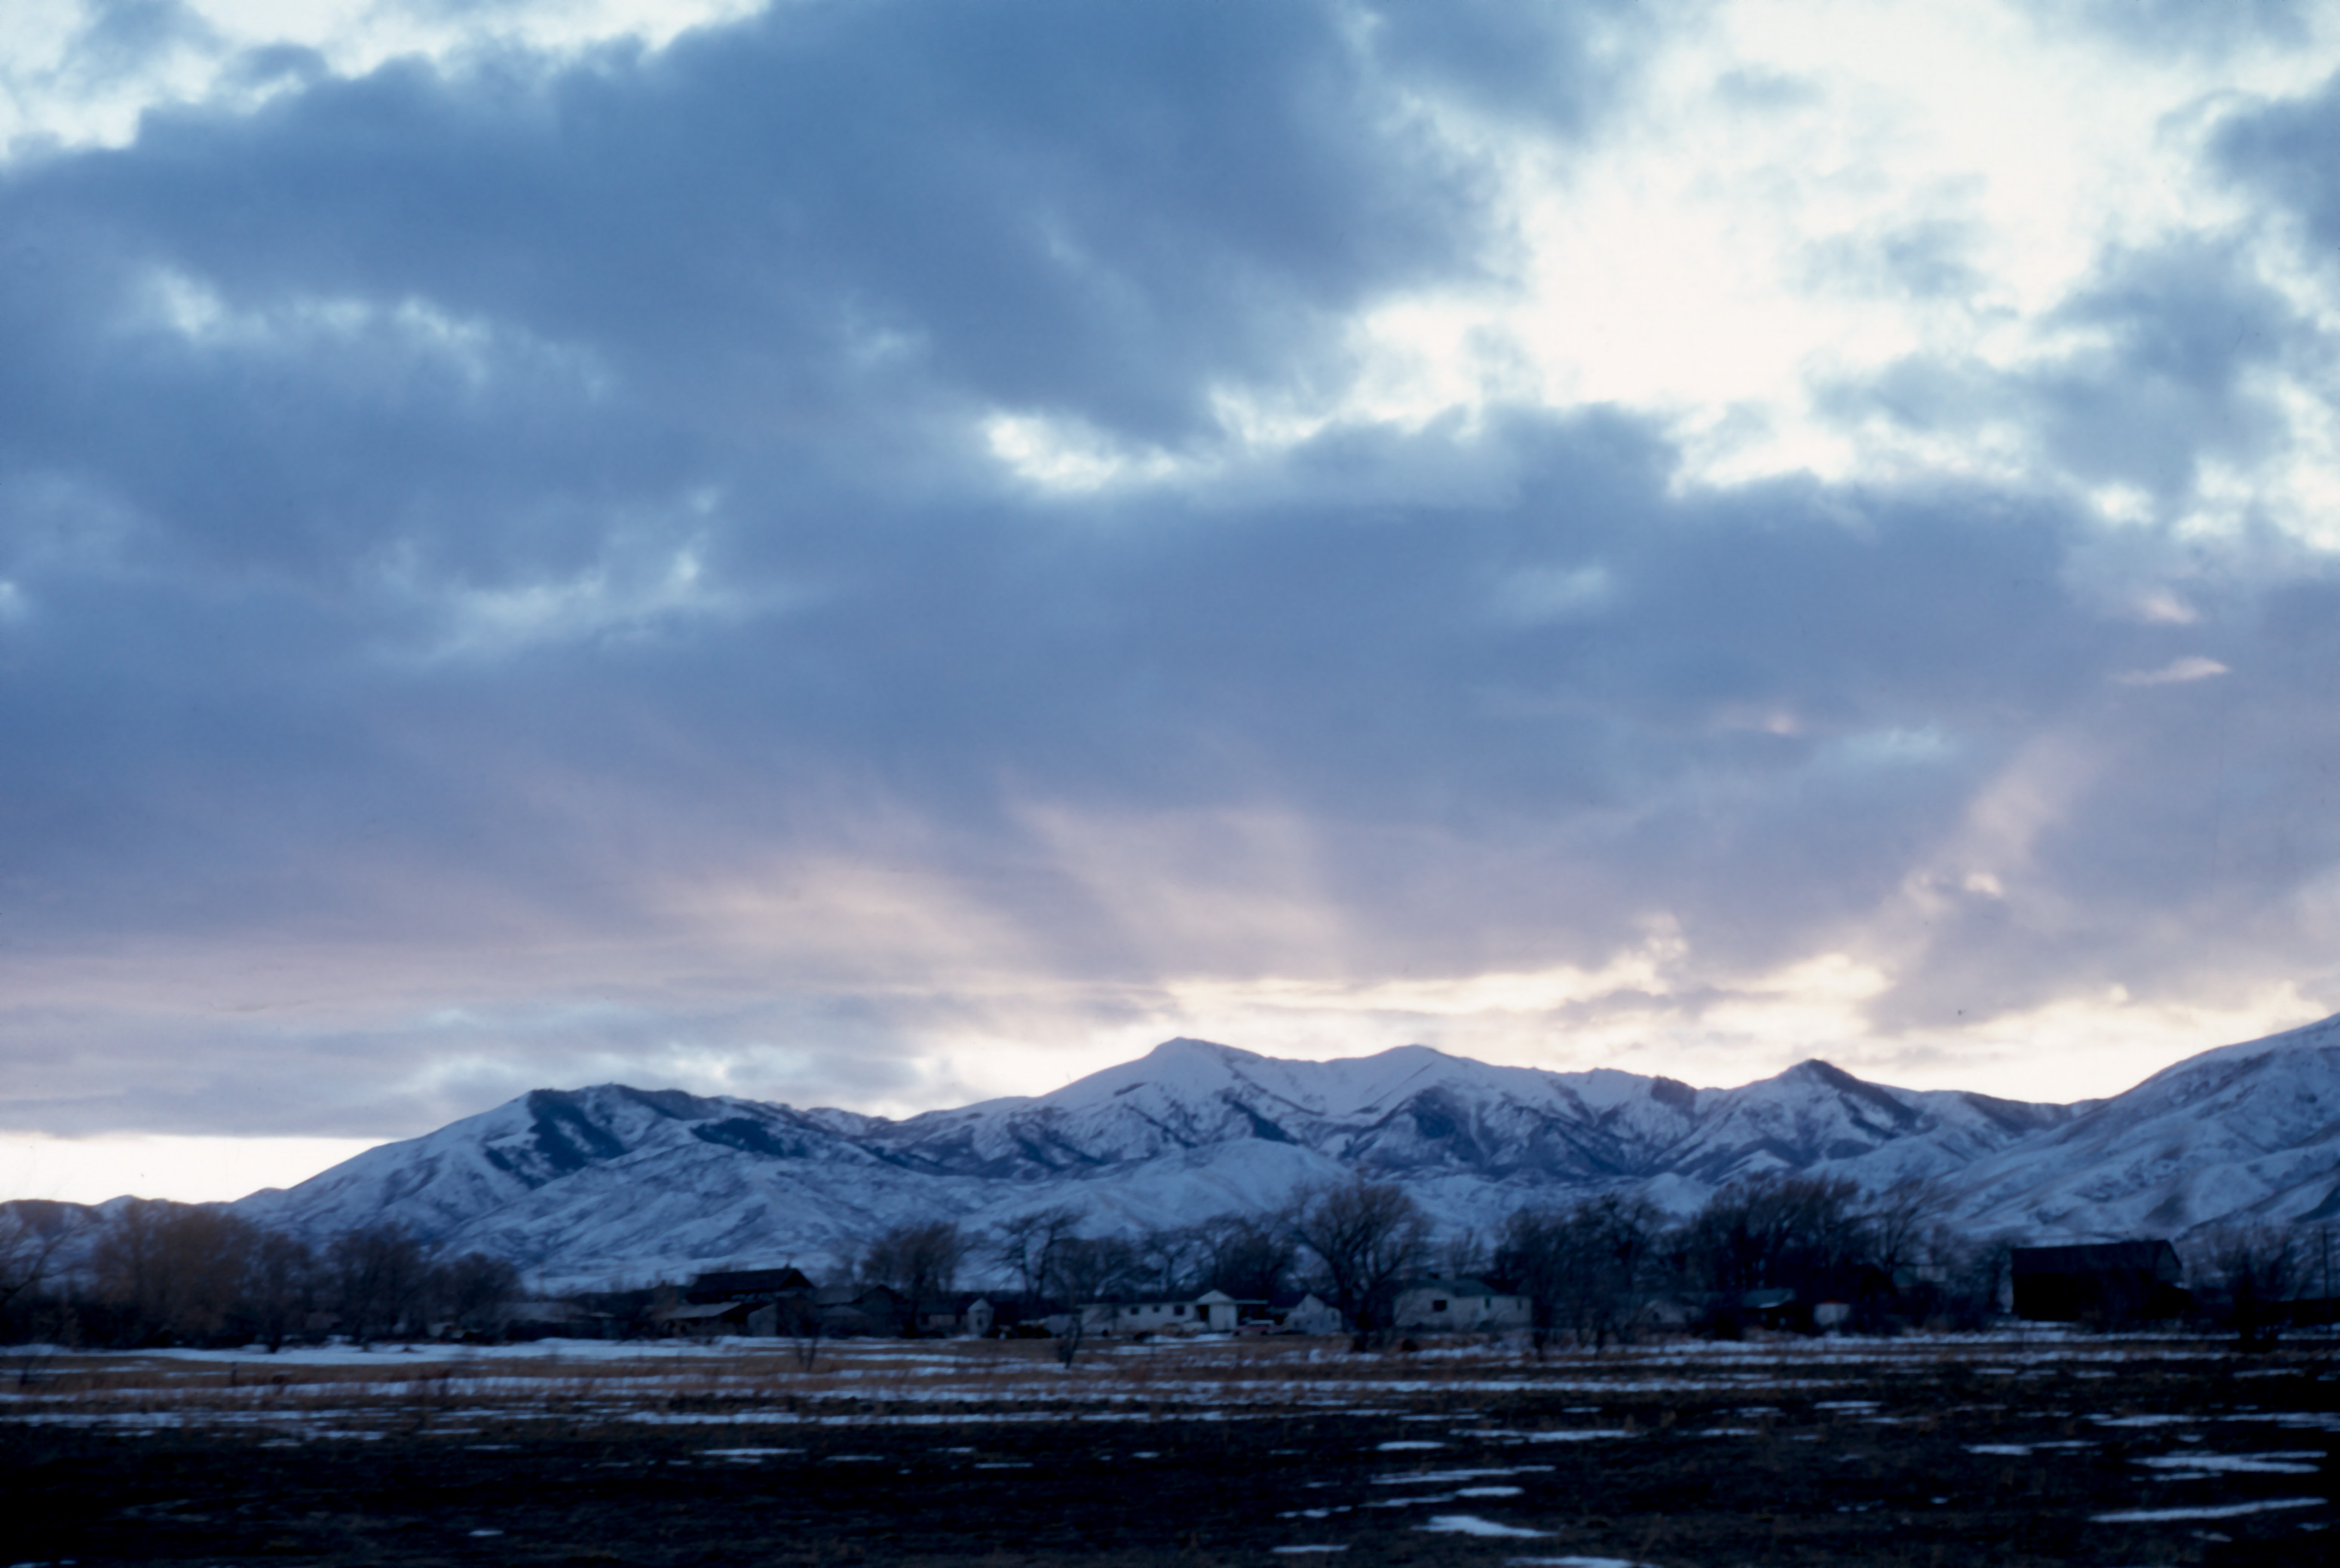
\includegraphics[width=\linewidth,height=\textheight,keepaspectratio]{/home/mkg/Dropbox/images/c-2013-03-12_12-07-24.jpg}
    \captionlistentry[figure]{\url{\protect\detokenize{This is a scan of the first picture I took that I actually liked, a 35 mm slide. It was in 1968 in the back yard of my father's girlfriend Doreen's house in Taylorsville, Utah, just after sunset. I believe this was Christmas Day.}}}
\end{figure}

\KOMAoptions{pagesize}
\clearpage
\recalctypearea
\newpage
\noindent
Filename: Date taken: GPS longitude: GPS latitude: Make: Model: Focal length (35mm eq): Exposure: F stop: ISO: Width: Height: 
\clearpage
\recalctypearea
\newpage
\noindent
\begin{figure}
    \includegraphics[width=\linewidth,height=\textheight,keepaspectratio]{/home/mkg/Dropbox/images/Mick, Wendy, Jane, Michael XMas.jpg}
    \captionlistentry[figure]{\url{\protect\detokenize{Scan of a slide of my grandfather Milton (Mick) Swensen, my sister Wendy, my grandmother Jane, and myself, Murray, Utah, Christmas or New Years 1968 I think.}}}
\end{figure}

\KOMAoptions{pagesize}
\clearpage
\recalctypearea
\newpage
\noindent
Filename: None\\ 
Date taken: None\\ 
GPS longitude: None\\ 
GPS latitude: None\\ 
Make: Nikon\\ 
Model: Nikon SUPER COOLSCAN 5000 ED\\ 
Focal length (35mm eq): None\\ 
Exposure: None\\ 
F stop: None\\ 
ISO: None\\ 
Width: 5782\\ 
Height: 3946\\ 

\clearpage
\recalctypearea
\newpage
\noindent
\begin{figure}
    \includegraphics[width=\linewidth,height=\textheight,keepaspectratio]{/home/mkg/Dropbox/images/renamed/c 2013-03-11_04-41-39.1.jpg}
    \captionlistentry[figure]{\url{\protect\detokenize{Scan of a slide of Elaine Constable, to whom I was briefly married, First Avenue stairs, Salt Lake City, Utah, 1971.}}}
\end{figure}

\KOMAoptions{pagesize}
\clearpage
\recalctypearea
\newpage
\noindent
Filename: None\\ 
Date taken: None\\ 
GPS longitude: None\\ 
GPS latitude: None\\ 
Make: Nikon\\ 
Model: Nikon SUPER COOLSCAN 5000 ED\\ 
Focal length (35mm eq): None\\ 
Exposure: None\\ 
F stop: None\\ 
ISO: None\\ 
Width: 5782\\ 
Height: 3946\\ 

\clearpage
\recalctypearea
\newpage
\noindent
\begin{figure}
    \includegraphics[width=\linewidth,height=\textheight,keepaspectratio]{/home/mkg/Dropbox/images/renamed/c 2013-03-11_04-41-41.1.jpg}
    \captionlistentry[figure]{\url{\protect\detokenize{Scan of a slide, sidewalk leaves, South Temple Street, Salt Lake City, Utah, 1972.}}}
\end{figure}

\KOMAoptions{pagesize}
\clearpage
\recalctypearea
\newpage
\noindent
Filename: None\\ 
Date taken: None\\ 
GPS longitude: None\\ 
GPS latitude: None\\ 
Make: Nikon\\ 
Model: Nikon SUPER COOLSCAN 5000 ED\\ 
Focal length (35mm eq): None\\ 
Exposure: None\\ 
F stop: None\\ 
ISO: None\\ 
Width: 5782\\ 
Height: 3946\\ 

\clearpage
\recalctypearea
\newpage
\noindent
\begin{figure}
    \includegraphics[width=\linewidth,height=\textheight,keepaspectratio]{/home/mkg/Dropbox/images/renamed/c 2013-03-11_04-41-44.1.jpg}
    \captionlistentry[figure]{\url{\protect\detokenize{Scan of a slide, Capitol Hill, Salt Lake City, Utah, 1972.}}}
\end{figure}

\KOMAoptions{pagesize}
\clearpage
\recalctypearea
\newpage
\noindent
Filename: None\\ 
Date taken: None\\ 
GPS longitude: None\\ 
GPS latitude: None\\ 
Make: Nikon\\ 
Model: Nikon SUPER COOLSCAN 5000 ED\\ 
Focal length (35mm eq): None\\ 
Exposure: None\\ 
F stop: None\\ 
ISO: None\\ 
Width: 5782\\ 
Height: 3946\\ 

\clearpage
\recalctypearea
\newpage
\noindent
\begin{figure}
    \includegraphics[width=\linewidth,height=\textheight,keepaspectratio]{/home/mkg/Dropbox/images/renamed/c 2013-03-11_04-41-51.1.jpg}
    \captionlistentry[figure]{\url{\protect\detokenize{Scan of a slide, dry cleaners around the corner from where I lived after separating from Elaine, Salt Lake City, Utah, 1972.}}}
\end{figure}

\KOMAoptions{pagesize}
\clearpage
\recalctypearea
\newpage
\noindent
Filename: None\\ 
Date taken: None\\ 
GPS longitude: None\\ 
GPS latitude: None\\ 
Make: Nikon\\ 
Model: Nikon SUPER COOLSCAN 5000 ED\\ 
Focal length (35mm eq): None\\ 
Exposure: None\\ 
F stop: None\\ 
ISO: None\\ 
Width: 5782\\ 
Height: 3946\\ 

\clearpage
\recalctypearea
\newpage
\noindent
\begin{figure}
    \includegraphics[width=\linewidth,height=\textheight,keepaspectratio]{/home/mkg/Dropbox/images/renamed/c 2013-03-11_04-41-49.1.jpg}
    \captionlistentry[figure]{\url{\protect\detokenize{Scan of a slide, coin laundromat, Third Avenue, Salt Lake City, Utah, 1972 or so.}}}
\end{figure}

\KOMAoptions{pagesize}
\clearpage
\recalctypearea
\newpage
\noindent
Filename: None\\ 
Date taken: None\\ 
GPS longitude: None\\ 
GPS latitude: None\\ 
Make: Nikon\\ 
Model: Nikon SUPER COOLSCAN 5000 ED\\ 
Focal length (35mm eq): None\\ 
Exposure: None\\ 
F stop: None\\ 
ISO: None\\ 
Width: 5782\\ 
Height: 3946\\ 

\clearpage
\recalctypearea
\newpage
\noindent
\begin{figure}
    \includegraphics[width=\linewidth,height=\textheight,keepaspectratio]{/home/mkg/Dropbox/images/renamed/c 2013-03-11_04-26-23.1.jpg}
    \captionlistentry[figure]{\url{\protect\detokenize{Scan of a slide taken by a friend with my camera of myself on flute, free jazz jam in Loring Park, Minneapolis, Minnesota, 1973.}}}
\end{figure}

\KOMAoptions{pagesize}
\clearpage
\recalctypearea
\newpage
\noindent
Filename: None\\ 
Date taken: None\\ 
GPS longitude: None\\ 
GPS latitude: None\\ 
Make: Nikon\\ 
Model: Nikon SUPER COOLSCAN 5000 ED\\ 
Focal length (35mm eq): None\\ 
Exposure: None\\ 
F stop: None\\ 
ISO: None\\ 
Width: 5782\\ 
Height: 3946\\ 

\clearpage
\recalctypearea
\newpage
\noindent
\begin{figure}
    \includegraphics[width=\linewidth,height=\textheight,keepaspectratio]{/home/mkg/Dropbox/images/renamed/c 2013-03-11_04-41-56.1.jpg}
    \captionlistentry[figure]{\url{\protect\detokenize{Scan of a slide of my sister Wendy, outside our building in the Loring Park neighborhood, Minneapolis, Minnesota, 1973.}}}
\end{figure}

\KOMAoptions{pagesize}
\clearpage
\recalctypearea
\newpage
\noindent
Filename: None\\ 
Date taken: None\\ 
GPS longitude: None\\ 
GPS latitude: None\\ 
Make: Nikon\\ 
Model: Nikon SUPER COOLSCAN 5000 ED\\ 
Focal length (35mm eq): None\\ 
Exposure: None\\ 
F stop: None\\ 
ISO: None\\ 
Width: 5782\\ 
Height: 3946\\ 

\clearpage
\recalctypearea
\newpage
\noindent
\begin{figure}
    \includegraphics[width=\linewidth,height=\textheight,keepaspectratio]{/home/mkg/Dropbox/images/renamed/c 2013-03-11_04-41-52.1.jpg}
    \captionlistentry[figure]{\url{\protect\detokenize{Scan of a slide, Bike on porch, Lake Harriet neighborhood, Minneapolis, Minnesota, 1973.}}}
\end{figure}

\KOMAoptions{pagesize}
\clearpage
\recalctypearea
\newpage
\noindent
Filename: None\\ 
Date taken: None\\ 
GPS longitude: None\\ 
GPS latitude: None\\ 
Make: Nikon\\ 
Model: Nikon SUPER COOLSCAN 5000 ED\\ 
Focal length (35mm eq): None\\ 
Exposure: None\\ 
F stop: None\\ 
ISO: None\\ 
Width: 5782\\ 
Height: 3946\\ 

\clearpage
\recalctypearea
\newpage
\noindent
\begin{figure}
    \includegraphics[width=\linewidth,height=\textheight,keepaspectratio]{/home/mkg/Dropbox/images/renamed/c 2013-03-11_04-41-57.1.jpg}
    \captionlistentry[figure]{\url{\protect\detokenize{Scan of a slide, my girlfriend Penny Suess, downtown Minneapolis, Minnesota, 1973.}}}
\end{figure}

\KOMAoptions{pagesize}
\clearpage
\recalctypearea
\newpage
\noindent
Filename: None\\ 
Date taken: None\\ 
GPS longitude: None\\ 
GPS latitude: None\\ 
Make: Nikon\\ 
Model: Nikon SUPER COOLSCAN 5000 ED\\ 
Focal length (35mm eq): None\\ 
Exposure: None\\ 
F stop: None\\ 
ISO: None\\ 
Width: 3946\\ 
Height: 5782\\ 

\clearpage
\recalctypearea
\newpage
\noindent
\begin{figure}
    \includegraphics[width=\linewidth,height=\textheight,keepaspectratio]{/home/mkg/Dropbox/images/renamed/c 2013-03-11_04-41-36.1.jpg}
    \captionlistentry[figure]{\url{\protect\detokenize{Scan of a slide taken at the Minnesota State Fair, 1973.}}}
\end{figure}

\KOMAoptions{pagesize}
\clearpage
\recalctypearea
\newpage
\noindent
Filename: None\\ 
Date taken: None\\ 
GPS longitude: None\\ 
GPS latitude: None\\ 
Make: Nikon\\ 
Model: Nikon SUPER COOLSCAN 5000 ED\\ 
Focal length (35mm eq): None\\ 
Exposure: None\\ 
F stop: None\\ 
ISO: None\\ 
Width: 5782\\ 
Height: 3946\\ 

\clearpage
\recalctypearea
\newpage
\noindent
\begin{figure}
    \includegraphics[width=\linewidth,height=\textheight,keepaspectratio]{/home/mkg/Dropbox/images/renamed/c 2013-03-11_04-41-58.1.jpg}
    \captionlistentry[figure]{\url{\protect\detokenize{Scan of a slide of my mother's sister Donna after Mick's funeral, on the street where she grew up, St. Paul, Minnesota, 1975.}}}
\end{figure}

\KOMAoptions{pagesize}
\clearpage
\recalctypearea
\newpage
\noindent
Filename: Date taken: GPS longitude: GPS latitude: Make: Model: Focal length (35mm eq): Exposure: F stop: ISO: Width: Height: 
\clearpage
\recalctypearea
\newpage
\noindent
\begin{figure}
    \includegraphics[width=\linewidth,height=\textheight,keepaspectratio]{/home/mkg/Dropbox/images/renamed/c 2013-03-11_04-26-24.2.jpg}
    \captionlistentry[figure]{\url{\protect\detokenize{Scan of a slide, eastern side of Mount Timpanogos, Wasatch Mountains, Utah, 1977.}}}
\end{figure}

\KOMAoptions{pagesize}
\clearpage
\recalctypearea
\newpage
\noindent
Filename: None\\ 
Date taken: None\\ 
GPS longitude: None\\ 
GPS latitude: None\\ 
Make: Nikon\\ 
Model: Nikon SUPER COOLSCAN 5000 ED\\ 
Focal length (35mm eq): None\\ 
Exposure: None\\ 
F stop: None\\ 
ISO: None\\ 
Width: 5782\\ 
Height: 3946\\ 

\clearpage
\recalctypearea
\newpage
\noindent
\begin{figure}
    \includegraphics[width=\linewidth,height=\textheight,keepaspectratio]{/home/mkg/Dropbox/images/renamed/c 2013-03-11_04-41-50.1.jpg}
    \captionlistentry[figure]{\url{\protect\detokenize{Scan of a slide of my girlfriend Esther's friend Merrie, Salt Lake City, Utah, 1977 or so.}}}
\end{figure}

\KOMAoptions{pagesize}
\clearpage
\recalctypearea
\newpage
\noindent
Filename: Date taken: GPS longitude: GPS latitude: Make: Model: Focal length (35mm eq): Exposure: F stop: ISO: Width: Height: 
\clearpage
\recalctypearea
\newpage
\noindent
\begin{figure}
    \includegraphics[width=\linewidth,height=\textheight,keepaspectratio]{/home/mkg/Dropbox/images/Jan 76P3 22 retouched.jpg}
    \captionlistentry[figure]{\url{\protect\detokenize{Scan of a slide of my cousin Jared and his then wife, Salt Lake City, Utah, 1976.}}}
\end{figure}

\KOMAoptions{pagesize}
\clearpage
\recalctypearea
\newpage
\noindent
Filename: None\\ 
Date taken: 2013:03:12 12:22:48\\ 
GPS longitude: None\\ 
GPS latitude: None\\ 
Make: Nikon\\ 
Model: Nikon SUPER COOLSCAN 5000 ED\\ 
Focal length (35mm eq): None\\ 
Exposure: None\\ 
F stop: None\\ 
ISO: None\\ 
Width: 5782\\ 
Height: 3946\\ 

\clearpage
\recalctypearea
\newpage
\noindent
\begin{figure}
    \includegraphics[width=\linewidth,height=\textheight,keepaspectratio]{/home/mkg/Dropbox/images/renamed/c 2013-03-12_12-22-47.jpg}
    \captionlistentry[figure]{\url{\protect\detokenize{Scan of a slide of Ruby Francis, Salt Lake City, Utah, I think in 1977.}}}
\end{figure}

\KOMAoptions{pagesize}
\clearpage
\recalctypearea
\newpage
\noindent
Filename: None\\ 
Date taken: None\\ 
GPS longitude: None\\ 
GPS latitude: None\\ 
Make: Nikon\\ 
Model: Nikon SUPER COOLSCAN 5000 ED\\ 
Focal length (35mm eq): None\\ 
Exposure: None\\ 
F stop: None\\ 
ISO: None\\ 
Width: 5782\\ 
Height: 3946\\ 

\clearpage
\recalctypearea
\newpage
\noindent
\begin{figure}
    \includegraphics[width=\linewidth,height=\textheight,keepaspectratio]{/home/mkg/Dropbox/images/renamed/c 2013-03-11_04-41-46.1.jpg}
    \captionlistentry[figure]{\url{\protect\detokenize{Scan of a slide of Charlie Potts, poet, Salt Lake City, Utah, 1977 or so.}}}
\end{figure}

\KOMAoptions{pagesize}
\clearpage
\recalctypearea
\newpage
\noindent
Filename: None\\ 
Date taken: None\\ 
GPS longitude: None\\ 
GPS latitude: None\\ 
Make: Nikon\\ 
Model: Nikon SUPER COOLSCAN 5000 ED\\ 
Focal length (35mm eq): None\\ 
Exposure: None\\ 
F stop: None\\ 
ISO: None\\ 
Width: 5782\\ 
Height: 3946\\ 

\clearpage
\recalctypearea
\newpage
\noindent
\begin{figure}
    \includegraphics[width=\linewidth,height=\textheight,keepaspectratio]{/home/mkg/Dropbox/images/renamed/c 2013-03-11_04-41-47.1.jpg}
    \captionlistentry[figure]{\url{\protect\detokenize{Scan of a slide of Memory Grove Park, Salt Lake City, Utah, winter of 1977 or so.}}}
\end{figure}

\KOMAoptions{pagesize}
\clearpage
\recalctypearea
\newpage
\noindent
Filename: Date taken: GPS longitude: GPS latitude: Make: Model: Focal length (35mm eq): Exposure: F stop: ISO: Width: Height: 
\clearpage
\recalctypearea
\newpage
\noindent
\begin{figure}
    \includegraphics[width=\linewidth,height=\textheight,keepaspectratio]{/home/mkg/Dropbox/images/c 2016-04-06_21-05-56.1.jpg}
    \captionlistentry[figure]{\url{\protect\detokenize{Scan of a slide of the Deep Creek Mountains, western Utah, 1977 or 1978.}}}
\end{figure}

\KOMAoptions{pagesize}
\clearpage
\recalctypearea
\newpage
\noindent
Filename: None\\ 
Date taken: 2010:11:15 07:07:01\\ 
GPS longitude: None\\ 
GPS latitude: None\\ 
Make: Canon\\ 
Model: Canon PowerShot G7\\ 
Focal length (35mm eq): None\\ 
Exposure: 0.008\\ 
F stop: 3.2\\ 
ISO: None\\ 
Width: 3648\\ 
Height: 2736\\ 

\clearpage
\recalctypearea
\newpage
\noindent
\begin{figure}
    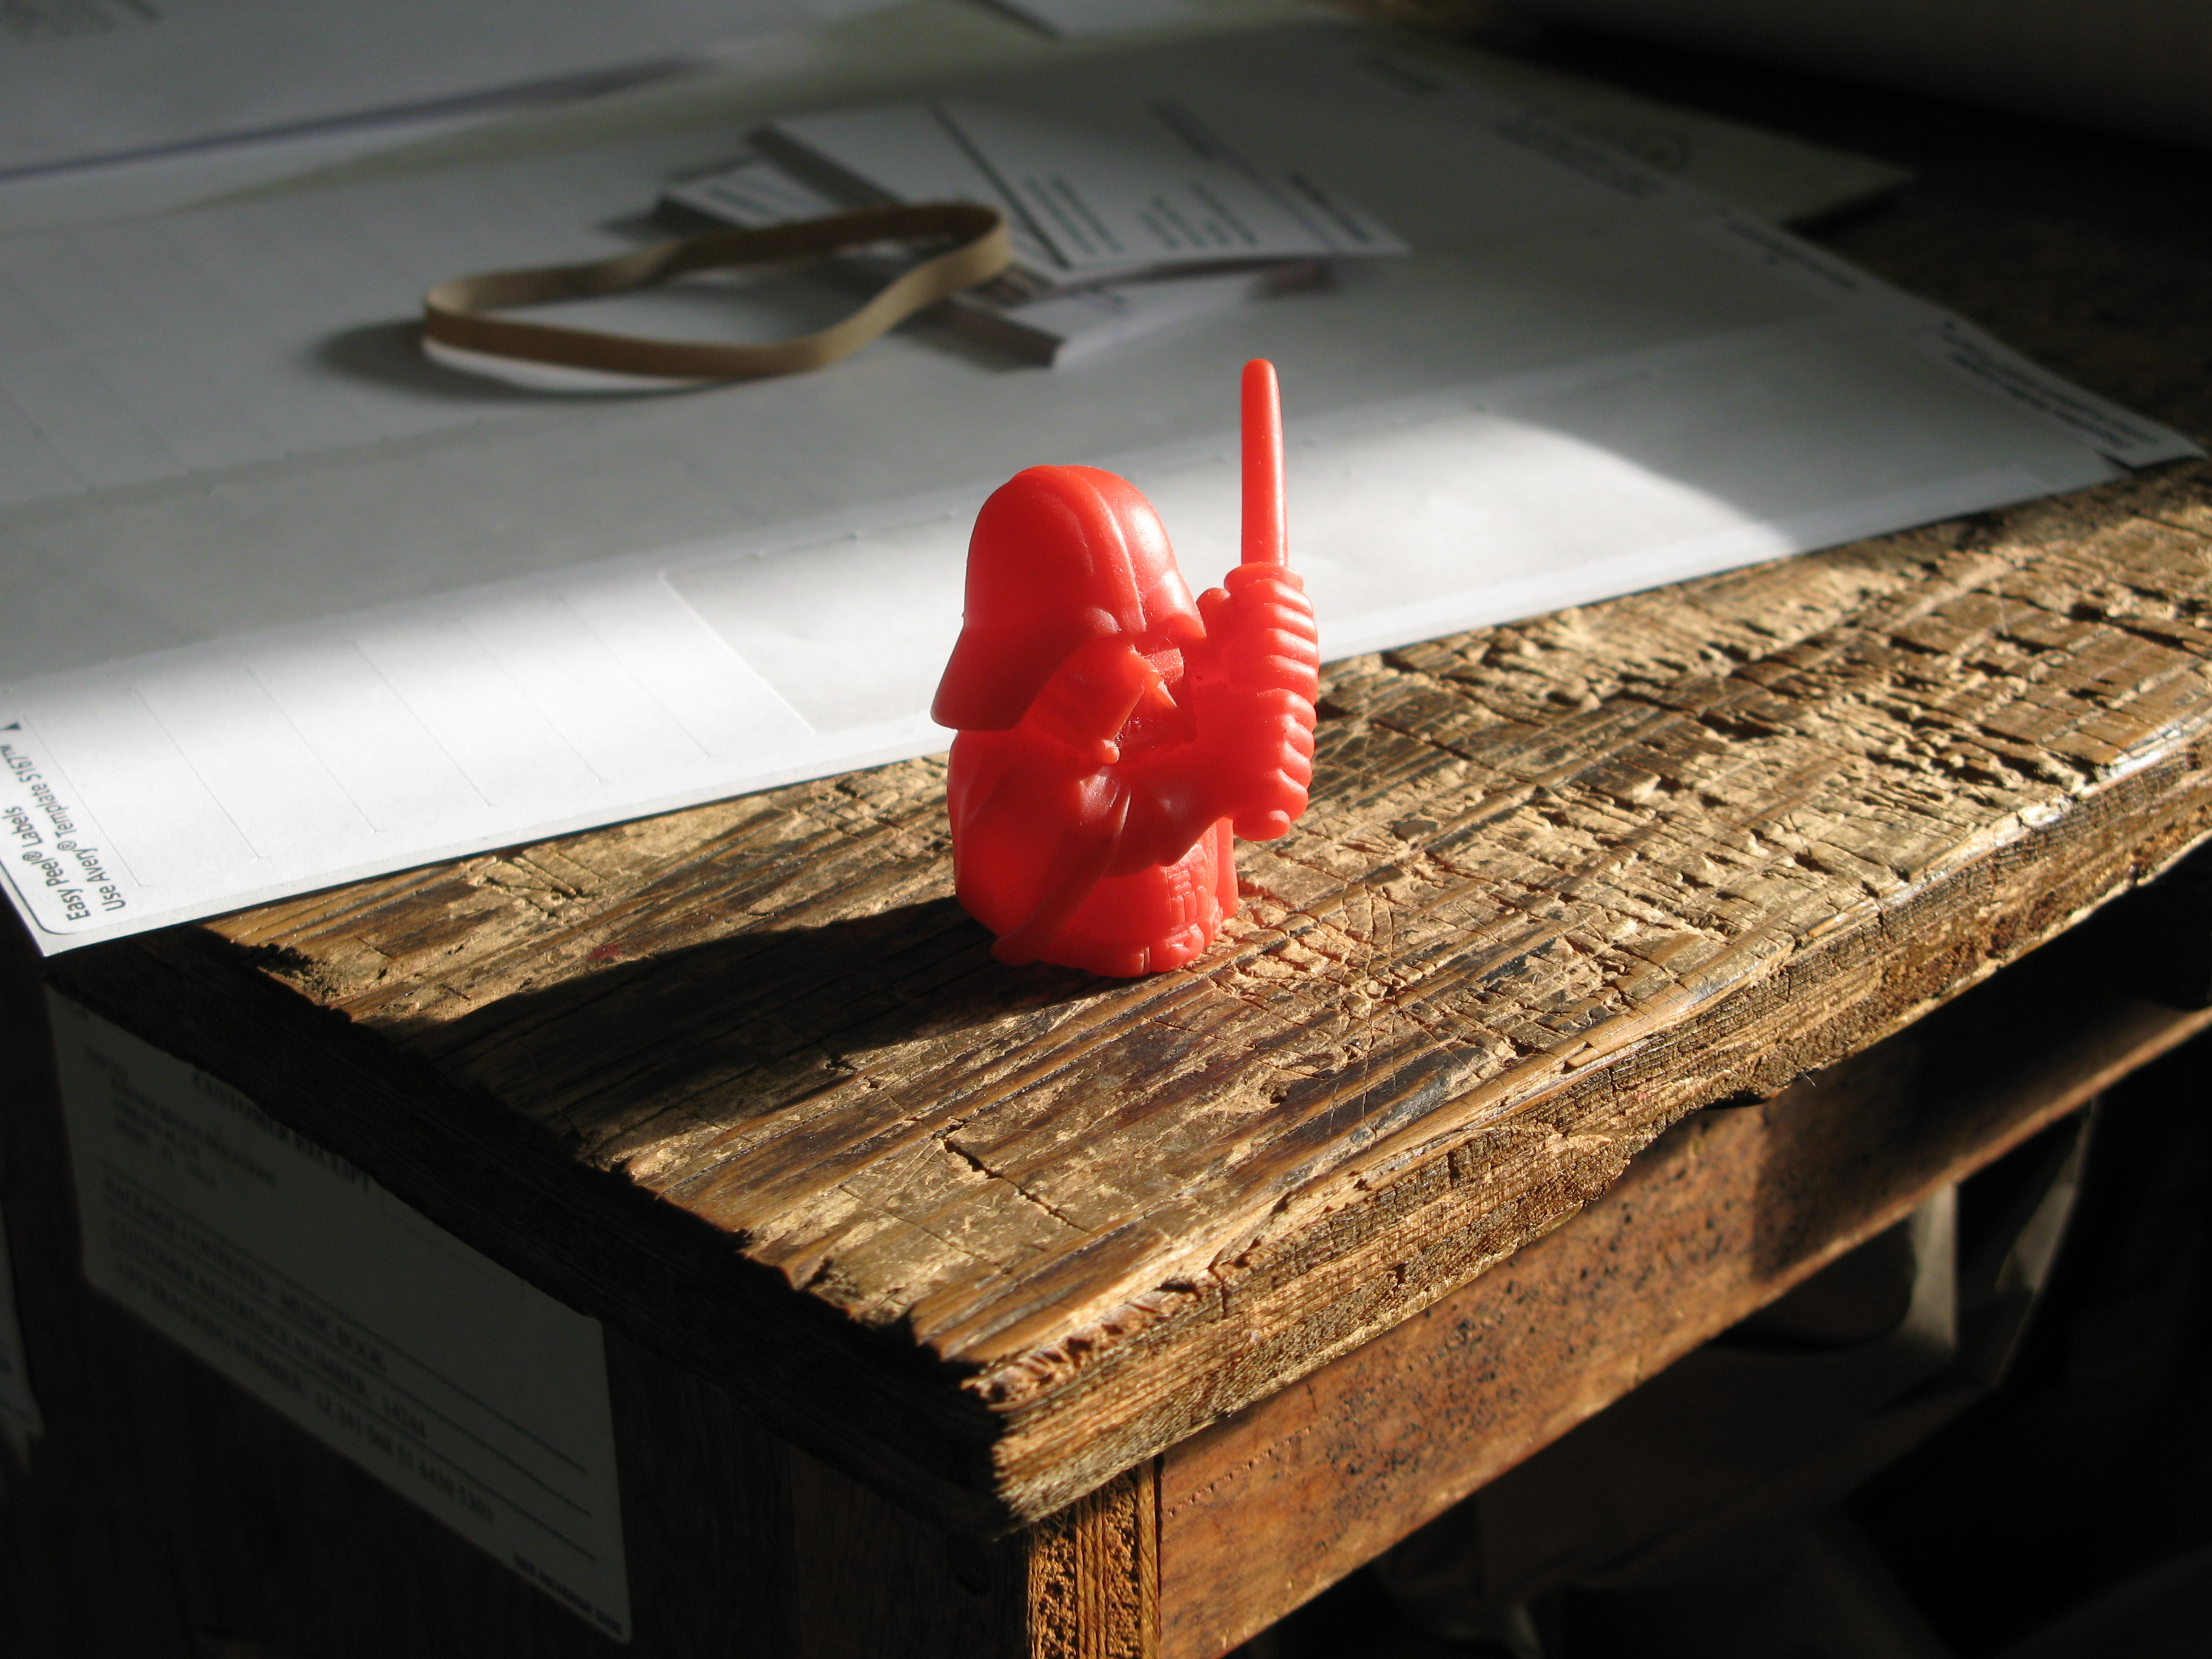
\includegraphics[width=\linewidth,height=\textheight,keepaspectratio]{/home/mkg/Dropbox/images/014.JPG}
    \captionlistentry[figure]{\url{\protect\detokenize{}}}
\end{figure}

\KOMAoptions{pagesize}
\clearpage
\recalctypearea
\newpage
\noindent
Filename: None\\ 
Date taken: 2005:07:31 05:51:04\\ 
GPS longitude: None\\ 
GPS latitude: None\\ 
Make: None\\ 
Model: None\\ 
Focal length (35mm eq): None\\ 
Exposure: None\\ 
F stop: None\\ 
ISO: None\\ 
Width: None\\ 
Height: None\\ 

\clearpage
\recalctypearea
\newpage
\noindent
\begin{figure}
    \includegraphics[width=\linewidth,height=\textheight,keepaspectratio]{/home/mkg/Dropbox/images/renamed/c 2013-03-11_04-26-22.1.jpg}
    \captionlistentry[figure]{\url{\protect\detokenize{Taken while hitchiking across the country.}}}
\end{figure}

\KOMAoptions{pagesize}
\clearpage
\recalctypearea
\newpage
\noindent
Filename: None\\ 
Date taken: None\\ 
GPS longitude: None\\ 
GPS latitude: None\\ 
Make: \\ 
Model: \\ 
Focal length (35mm eq): None\\ 
Exposure: None\\ 
F stop: None\\ 
ISO: ()\\ 
Width: 3160\\ 
Height: 2128\\ 

\clearpage
\recalctypearea
\newpage
\noindent
\begin{figure}
    \includegraphics[width=\linewidth,height=\textheight,keepaspectratio]{/home/mkg/Dropbox/images/Scan7.jpg}
    \captionlistentry[figure]{\url{\protect\detokenize{Scan of a slide of the Roman Forum.}}}
\end{figure}

\KOMAoptions{pagesize}
\clearpage
\recalctypearea
\newpage
\noindent
Filename: None\\ 
Date taken: 2002:01:01 00:00:00\\ 
GPS longitude: None\\ 
GPS latitude: None\\ 
Make: Minolta Co., Ltd.\\ 
Model: DiMAGE F100\\ 
Focal length (35mm eq): 90\\ 
Exposure: 0.004\\ 
F stop: 6.7\\ 
ISO: 100\\ 
Width: 2272\\ 
Height: 1704\\ 

\clearpage
\recalctypearea
\newpage
\noindent
\begin{figure}
    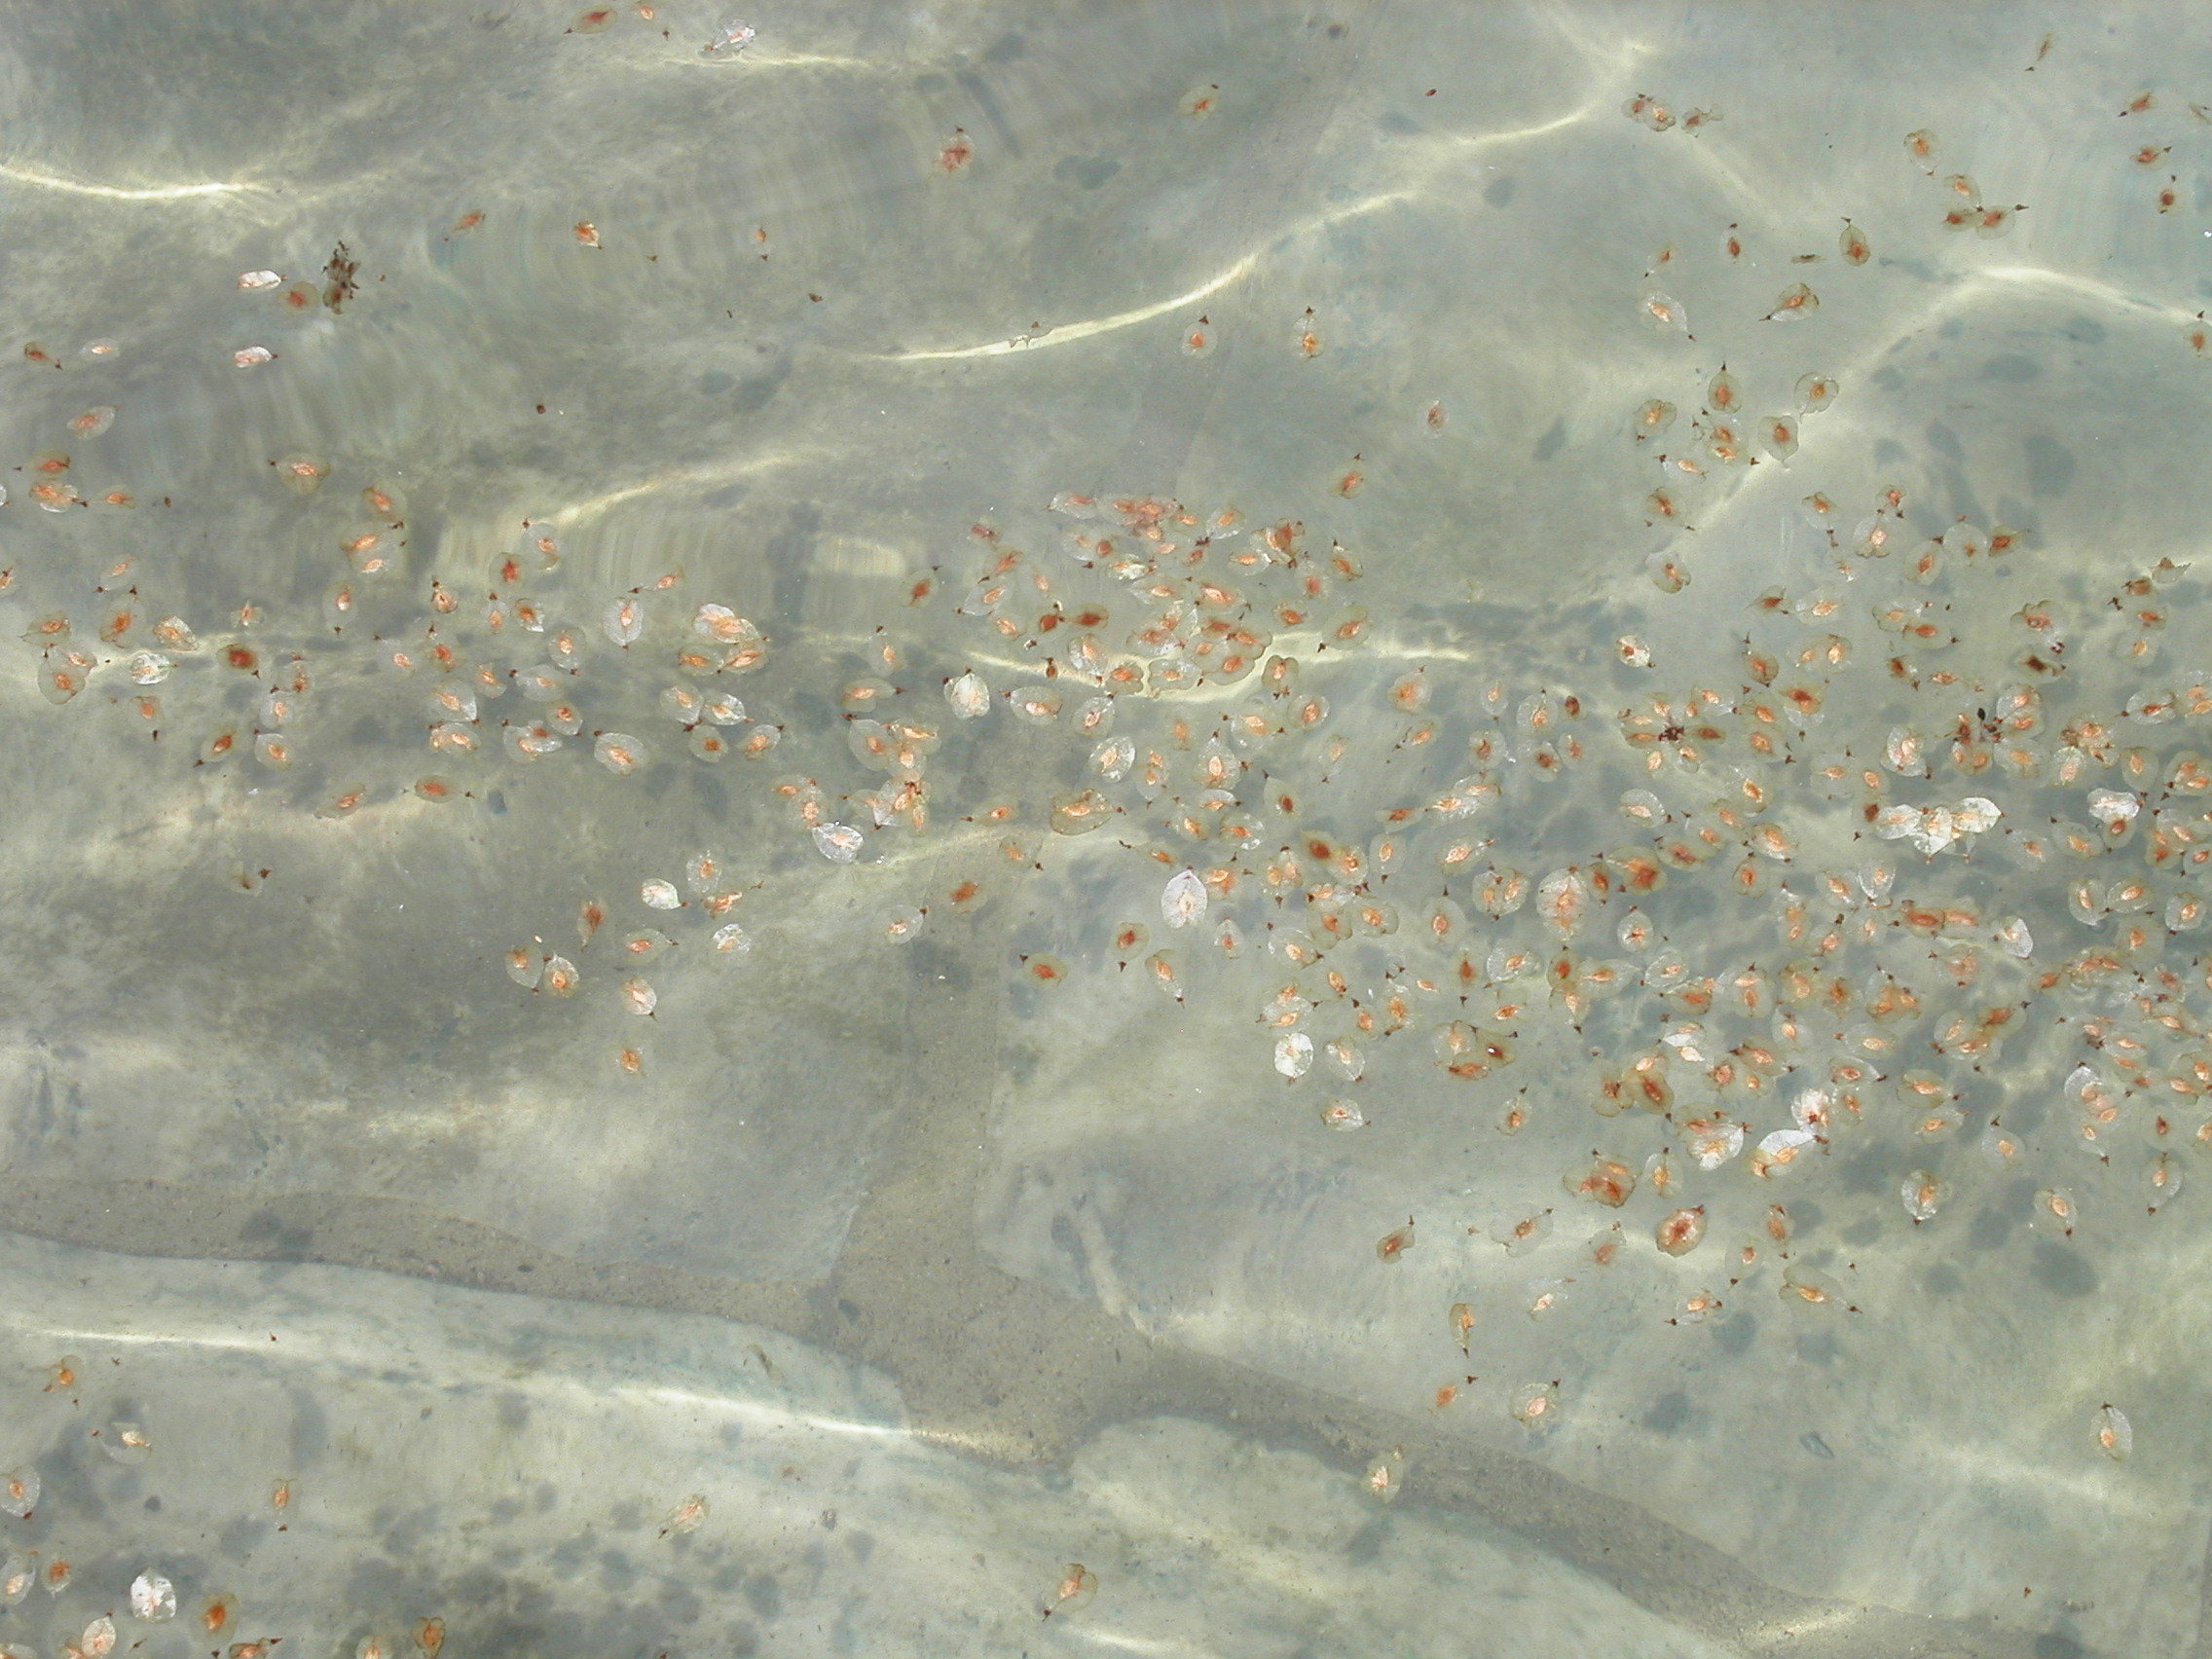
\includegraphics[width=\linewidth,height=\textheight,keepaspectratio]{/home/mkg/Dropbox/images/2004-04-13-b 010.jpg}
    \captionlistentry[figure]{\url{\protect\detokenize{}}}
\end{figure}

\KOMAoptions{pagesize}
\clearpage
\recalctypearea
\newpage
\noindent
Filename: None\\ 
Date taken: 2004:12:18 18:59:05\\ 
GPS longitude: None\\ 
GPS latitude: None\\ 
Make: OLYMPUS CORPORATION\\ 
Model: C8080WZ\\ 
Focal length (35mm eq): None\\ 
Exposure: 0.5\\ 
F stop: 2.5\\ 
ISO: 200\\ 
Width: 3264\\ 
Height: 2448\\ 

\clearpage
\recalctypearea
\newpage
\noindent
\begin{figure}
    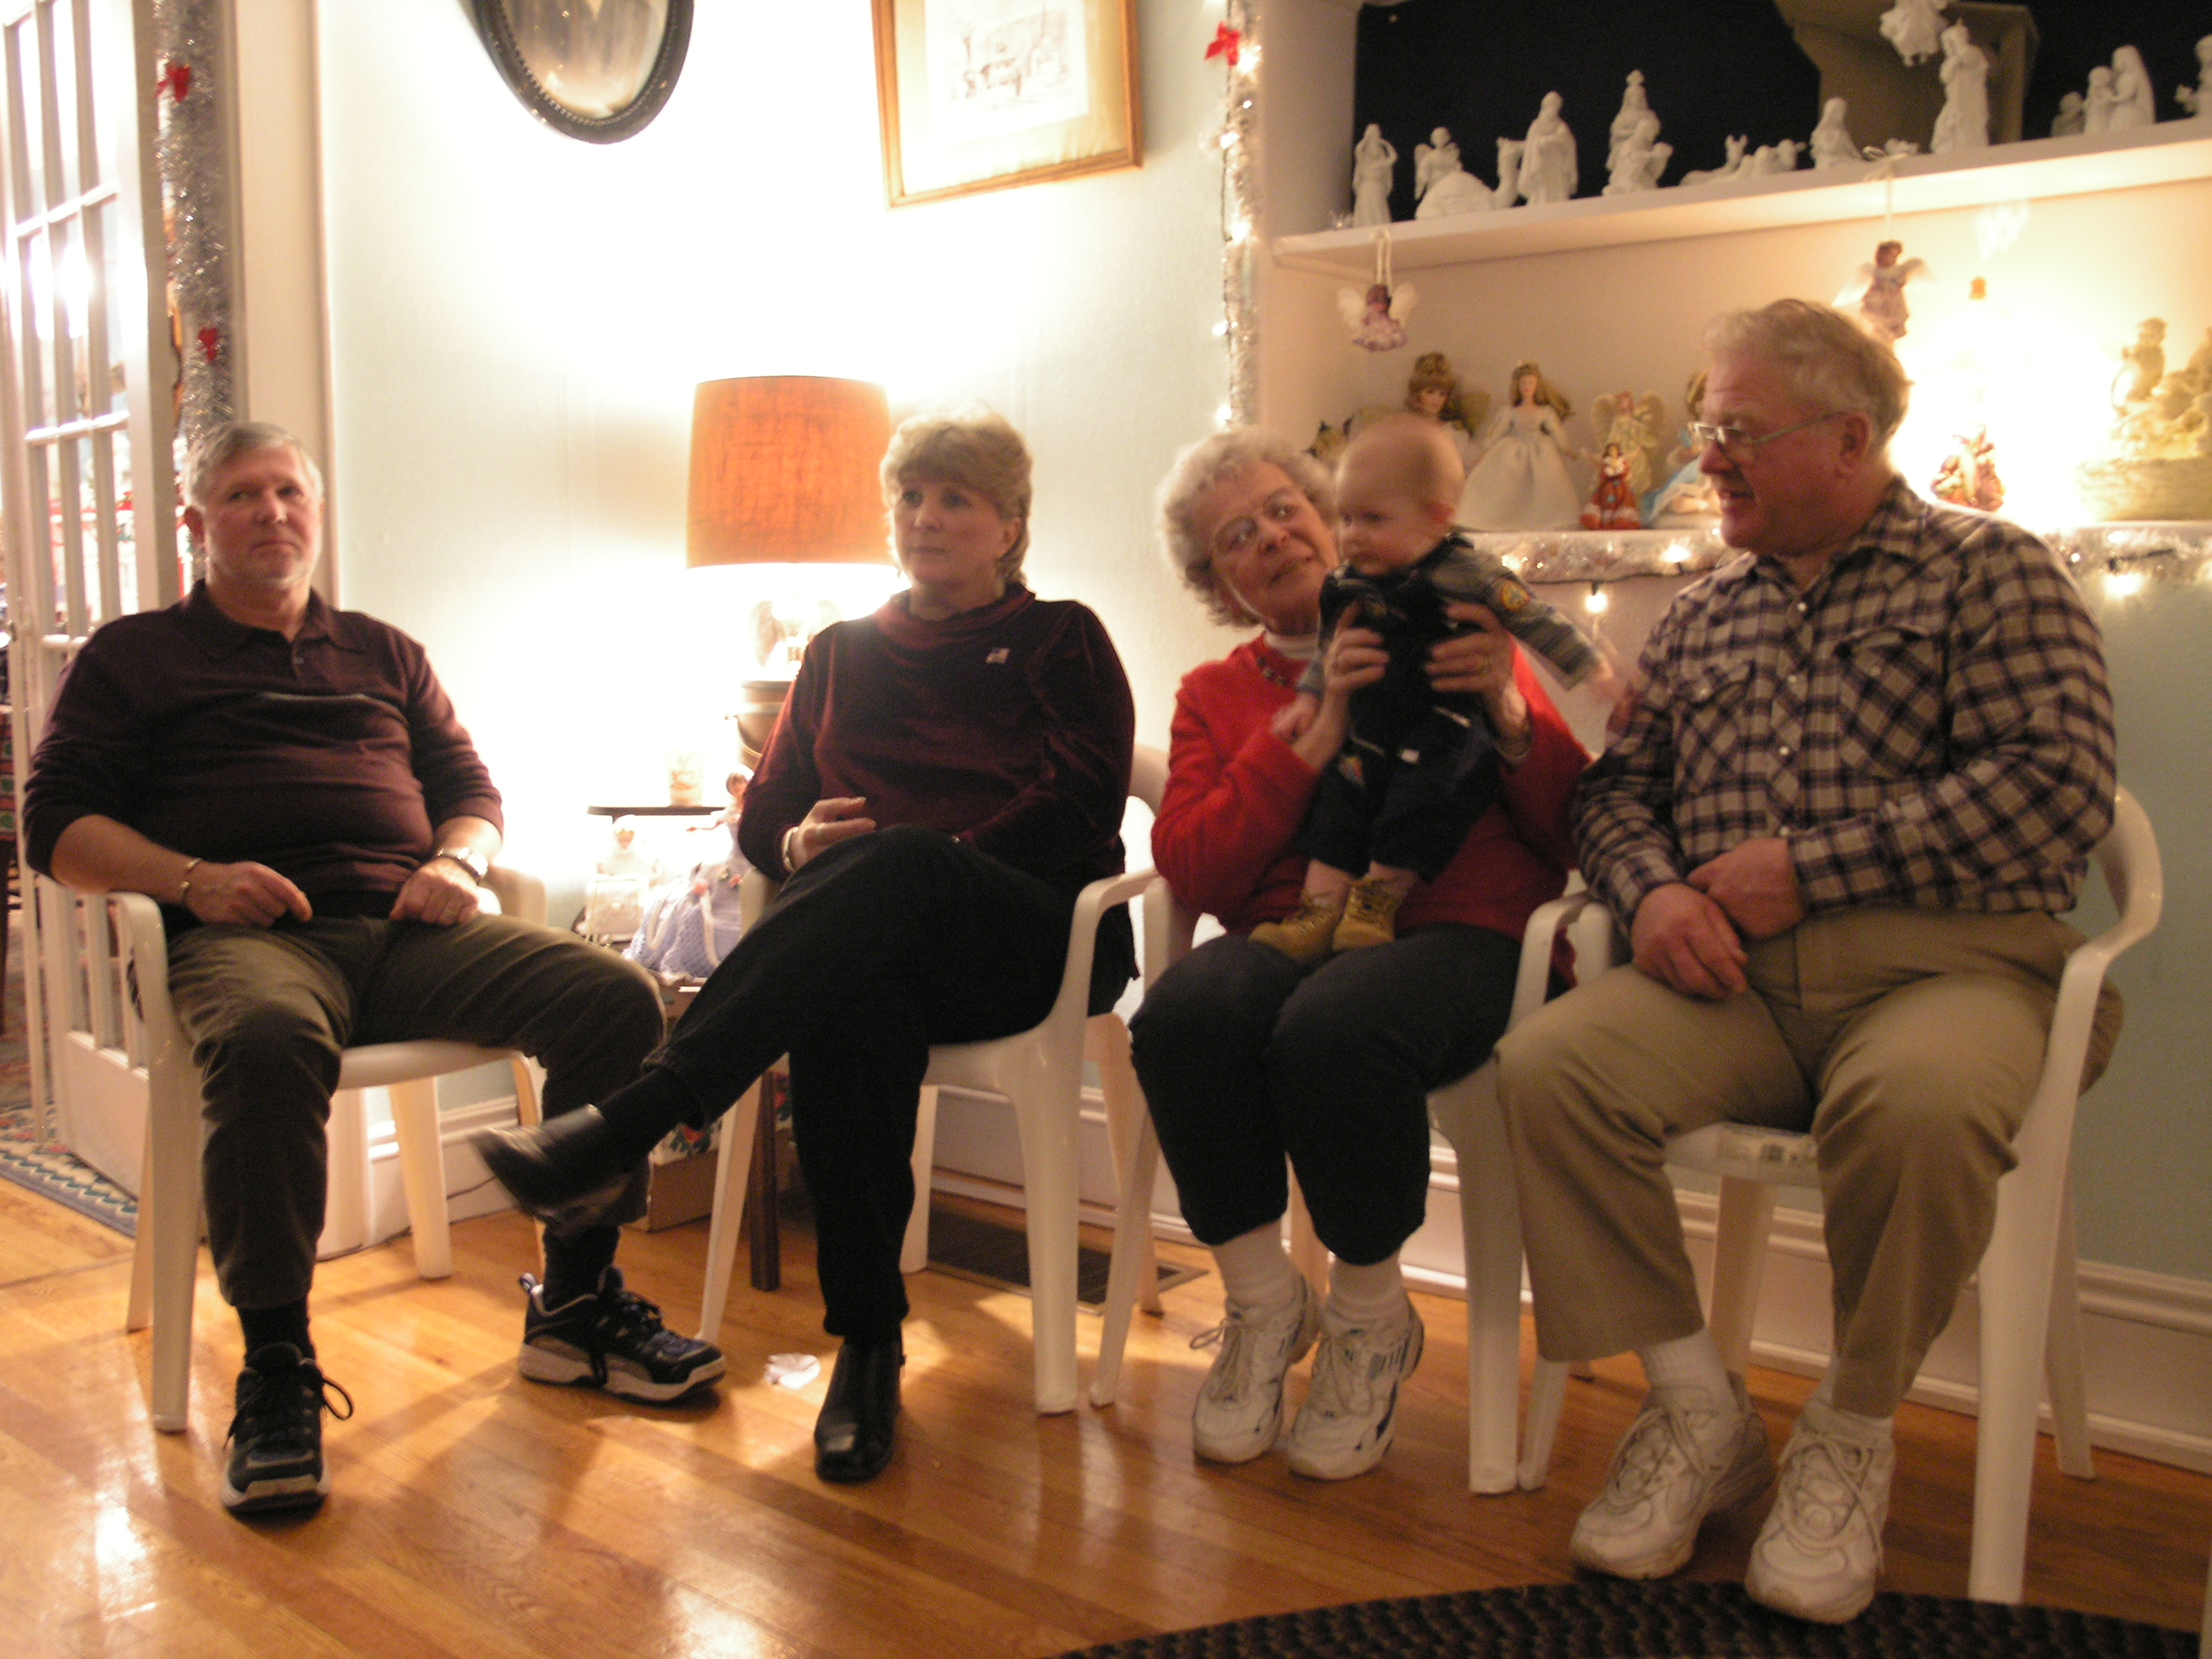
\includegraphics[width=\linewidth,height=\textheight,keepaspectratio]{/home/mkg/Dropbox/images/2004-12-18a 023.jpg}
    \captionlistentry[figure]{\url{\protect\detokenize{}}}
\end{figure}

\KOMAoptions{pagesize}
\clearpage
\recalctypearea
\newpage
\noindent
Filename: None\\ 
Date taken: 2004:12:18 19:00:08\\ 
GPS longitude: None\\ 
GPS latitude: None\\ 
Make: OLYMPUS CORPORATION\\ 
Model: C8080WZ\\ 
Focal length (35mm eq): None\\ 
Exposure: 0.4\\ 
F stop: 2.5\\ 
ISO: 200\\ 
Width: 3264\\ 
Height: 2448\\ 

\clearpage
\recalctypearea
\newpage
\noindent
\begin{figure}
    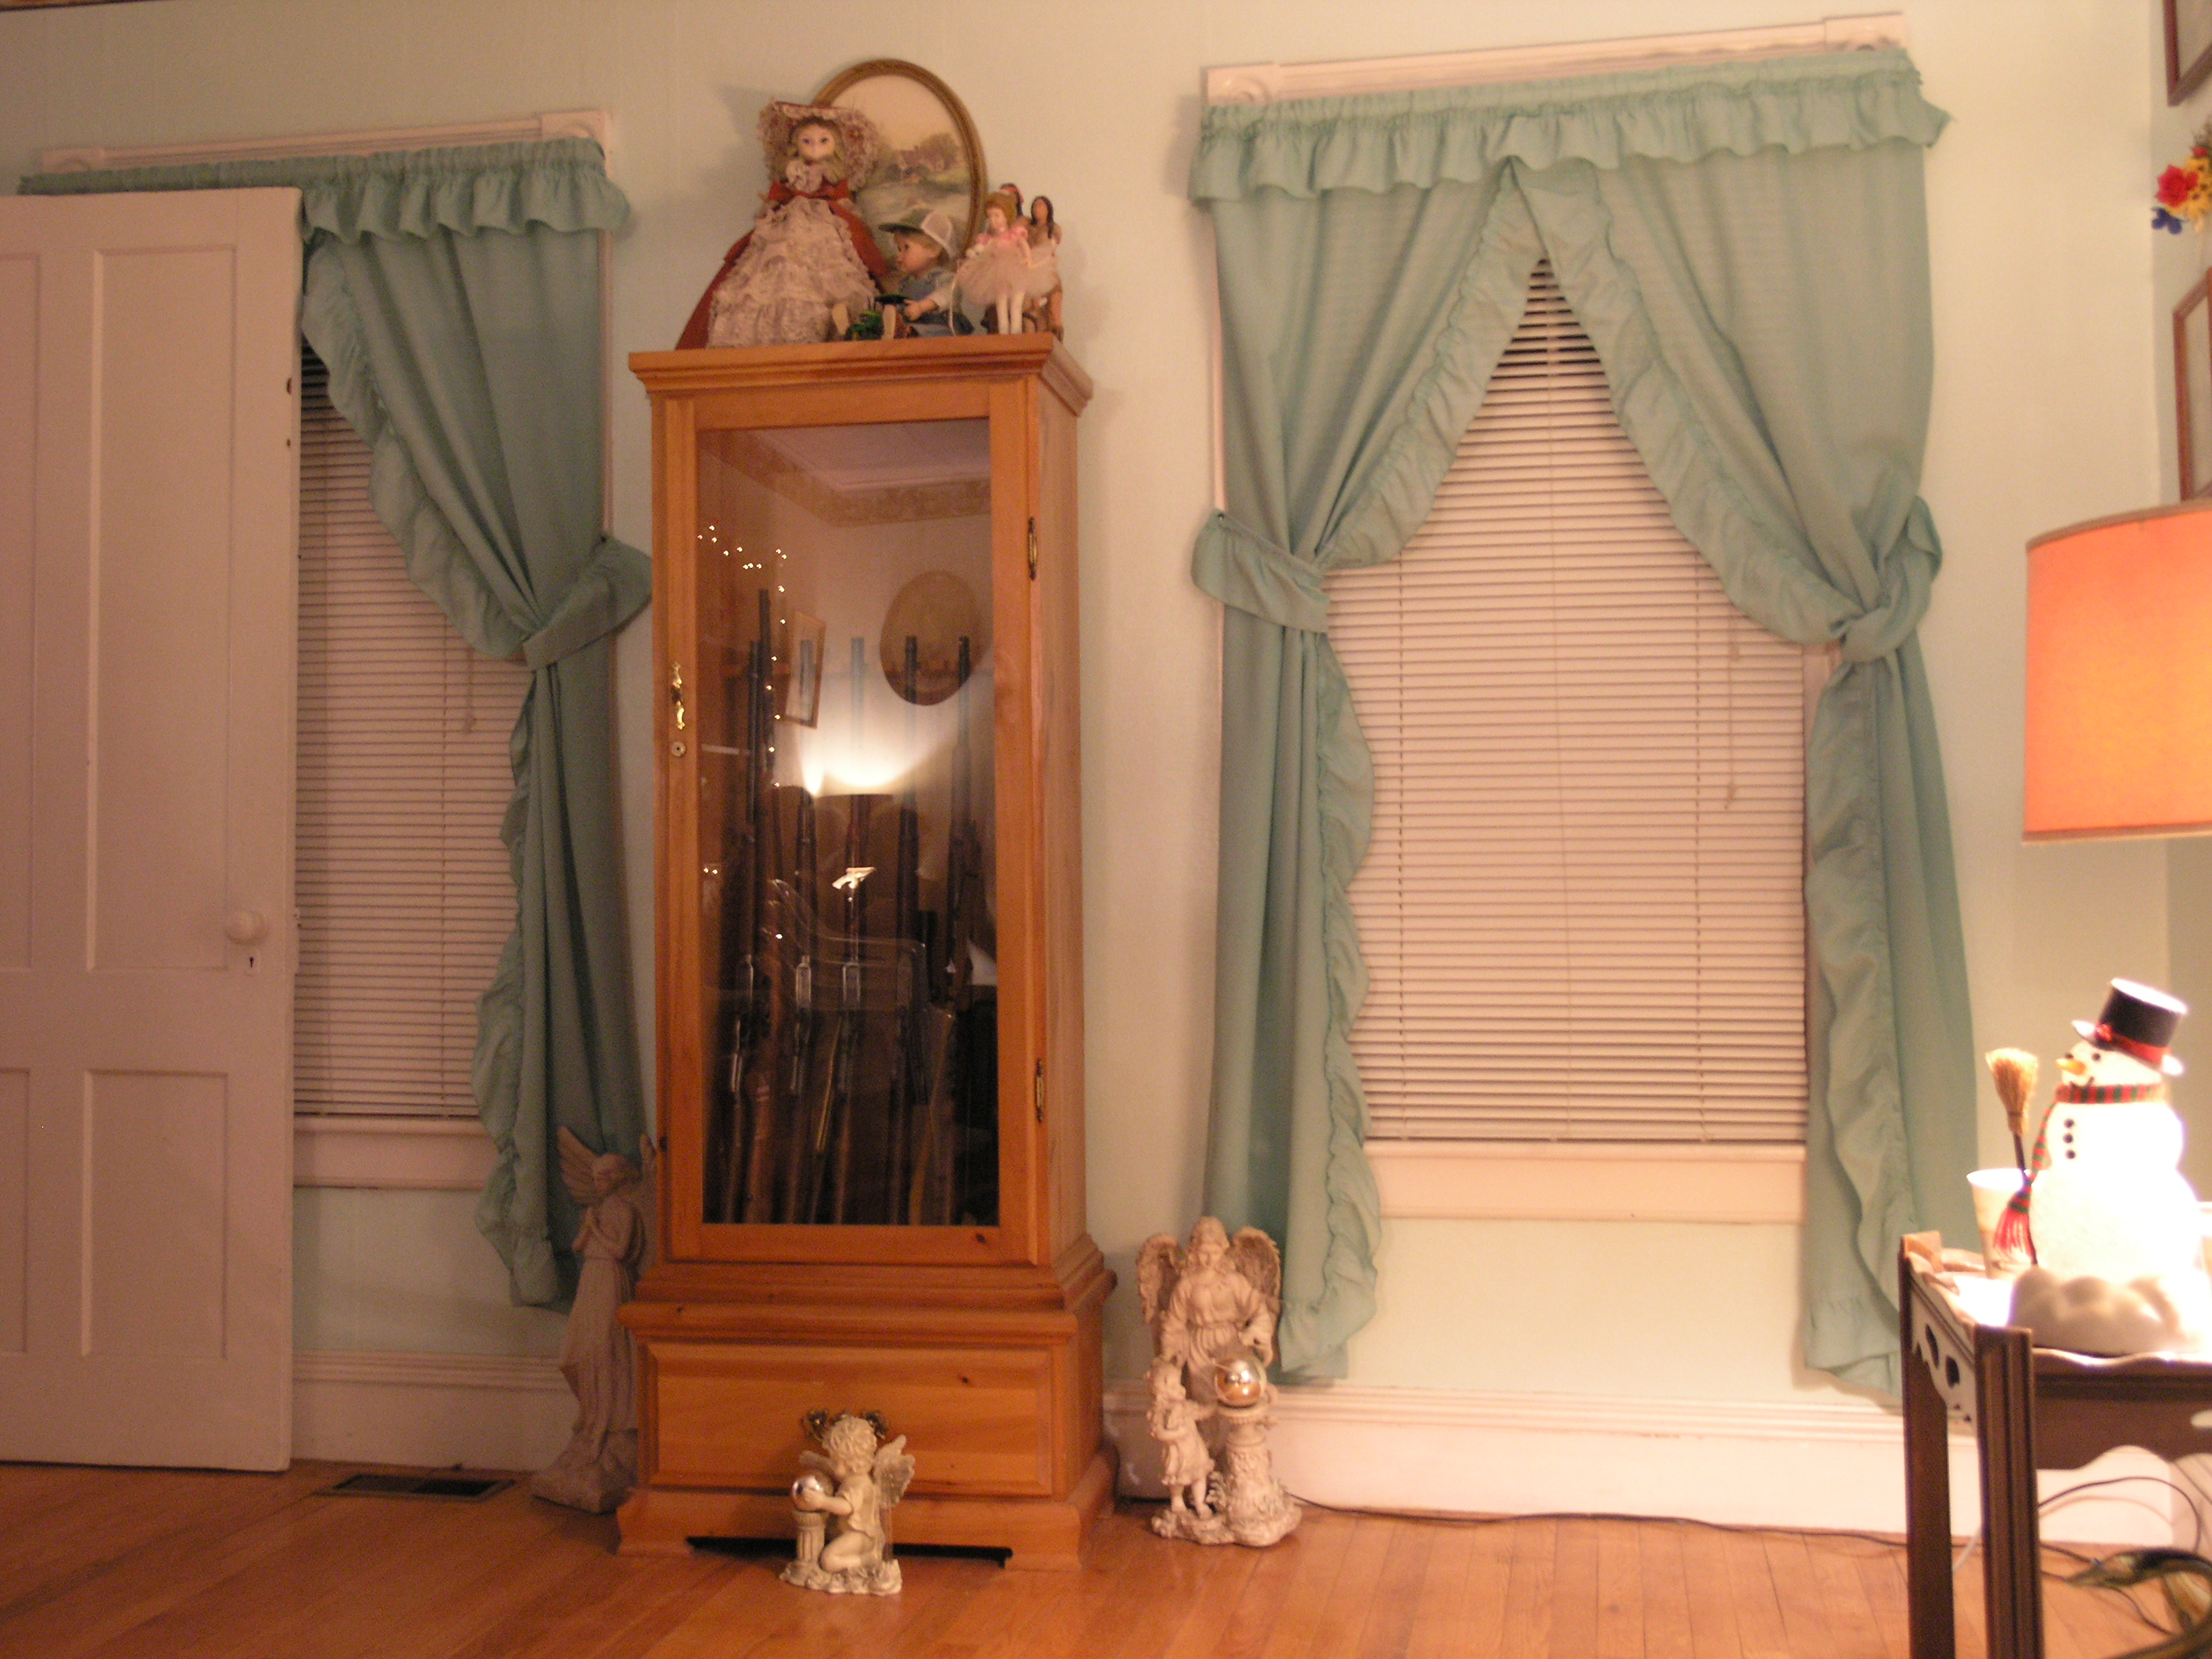
\includegraphics[width=\linewidth,height=\textheight,keepaspectratio]{/home/mkg/Dropbox/images/2004-12-18a 026.jpg}
    \captionlistentry[figure]{\url{\protect\detokenize{}}}
\end{figure}

\KOMAoptions{pagesize}
\clearpage
\recalctypearea
\newpage
\noindent
Filename: None\\ 
Date taken: 2005:01:15 09:31:36\\ 
GPS longitude: None\\ 
GPS latitude: None\\ 
Make: OLYMPUS CORPORATION\\ 
Model: C8080WZ\\ 
Focal length (35mm eq): None\\ 
Exposure: 0.008\\ 
F stop: 4.0\\ 
ISO: 50\\ 
Width: 3264\\ 
Height: 2448\\ 

\clearpage
\recalctypearea
\newpage
\noindent
\begin{figure}
    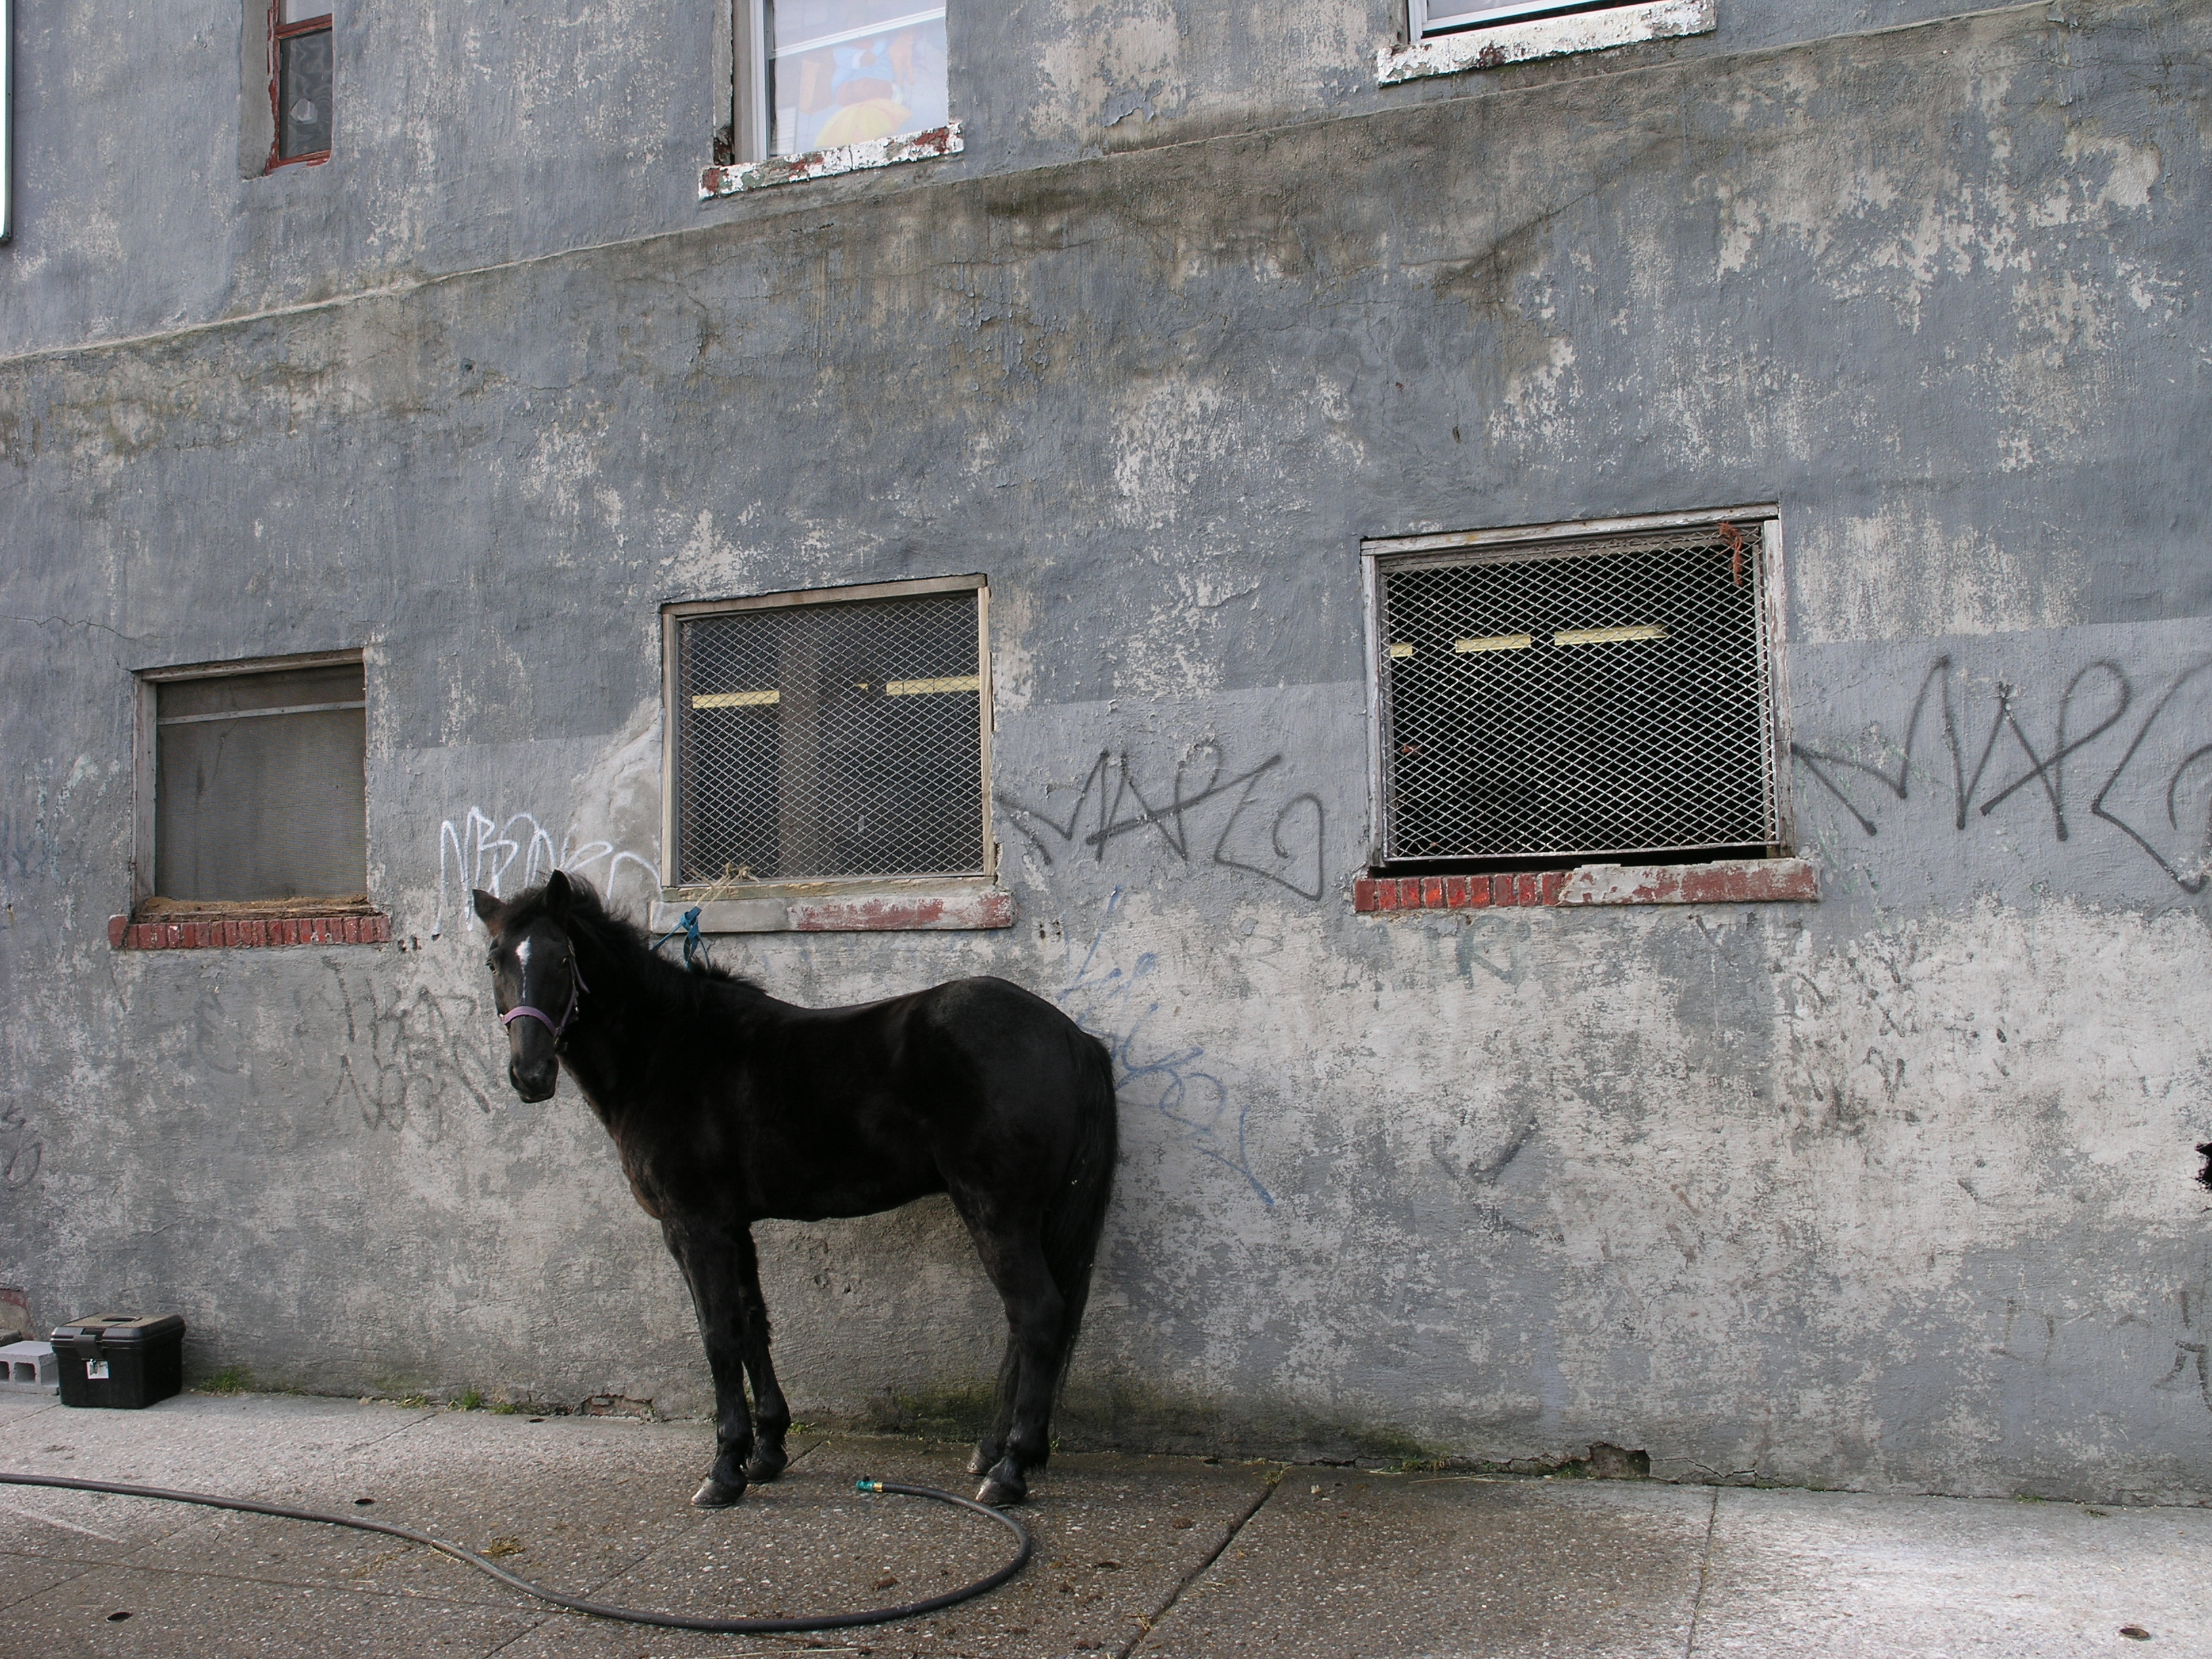
\includegraphics[width=\linewidth,height=\textheight,keepaspectratio]{/home/mkg/Dropbox/images/2005-02-28a 002.jpg}
    \captionlistentry[figure]{\url{\protect\detokenize{The only riding stable in Brooklyn.}}}
\end{figure}

\KOMAoptions{pagesize}
\clearpage
\recalctypearea
\newpage
\noindent
Filename: None\\ 
Date taken: 2005:05:04 18:21:50\\ 
GPS longitude: None\\ 
GPS latitude: None\\ 
Make: OLYMPUS CORPORATION\\ 
Model: C8080WZ\\ 
Focal length (35mm eq): None\\ 
Exposure: 0.016666666666666666\\ 
F stop: 3.5\\ 
ISO: 100\\ 
Width: 3264\\ 
Height: 2448\\ 

\clearpage
\recalctypearea
\newpage
\noindent
\begin{figure}
    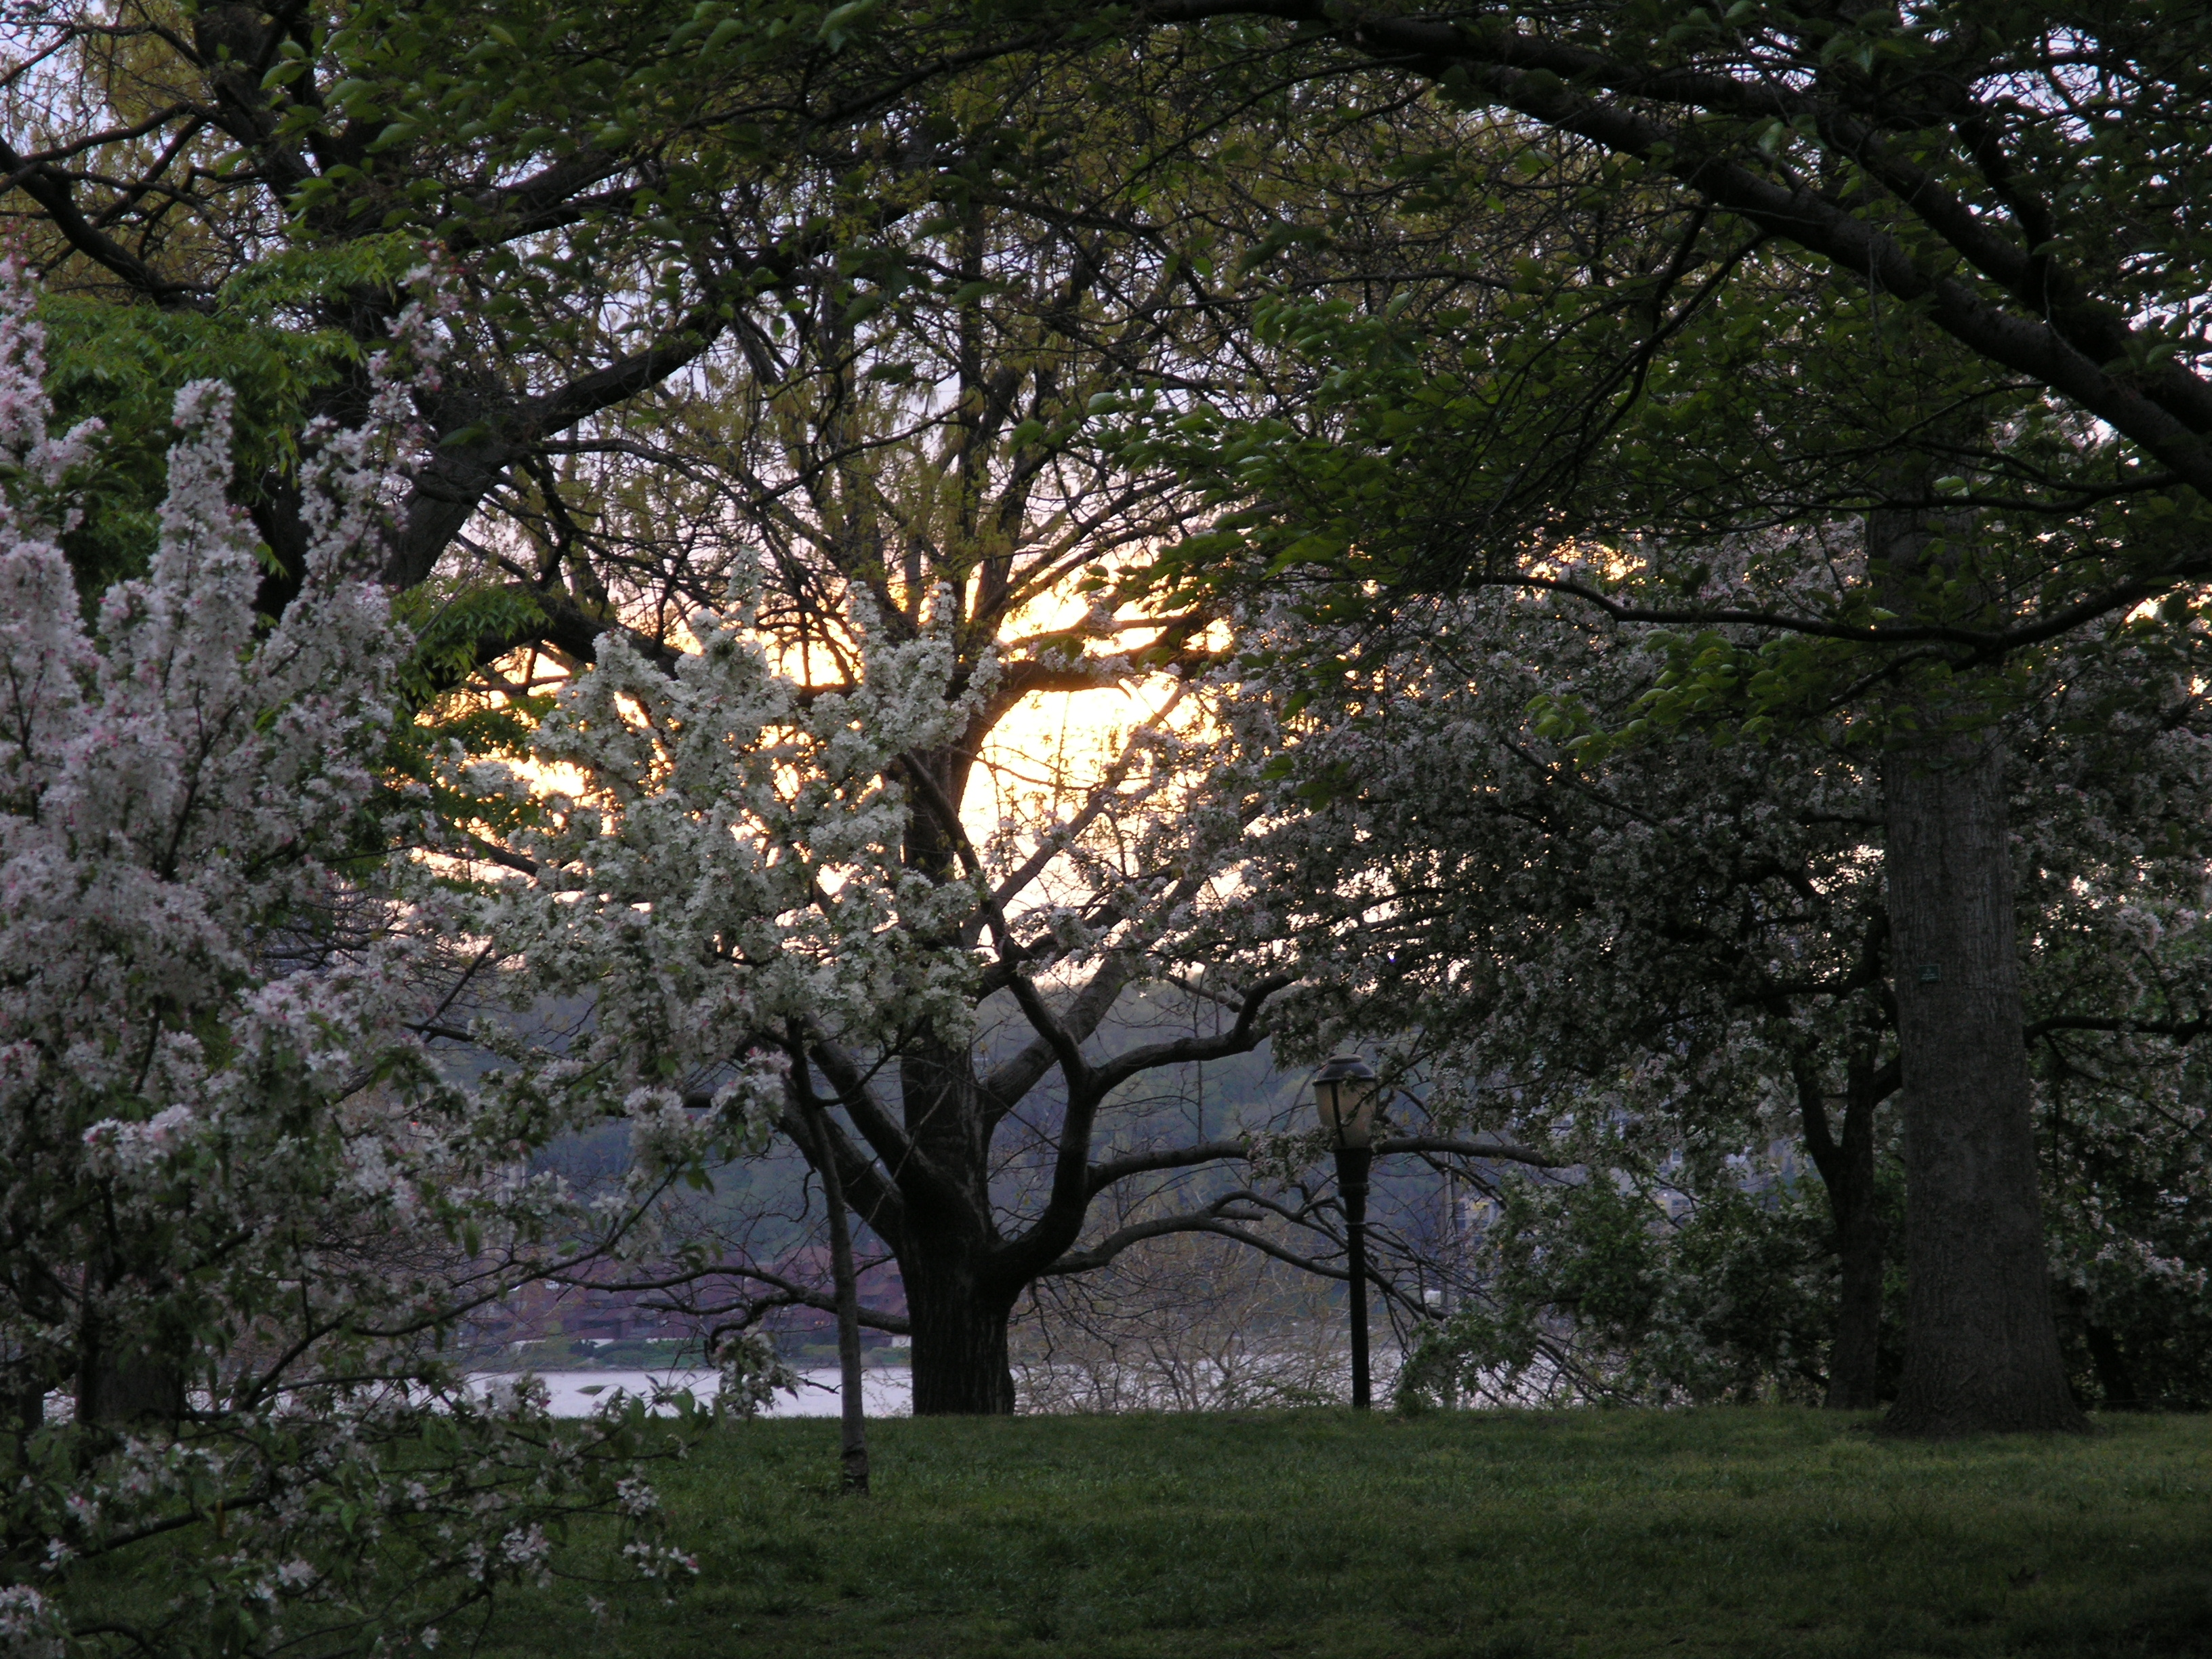
\includegraphics[width=\linewidth,height=\textheight,keepaspectratio]{/home/mkg/Dropbox/images/2005-05-17a 042.jpg}
    \captionlistentry[figure]{\url{\protect\detokenize{}}}
\end{figure}

\KOMAoptions{pagesize}
\clearpage
\recalctypearea
\newpage
\noindent
Filename: None\\ 
Date taken: 2005:07:09 09:38:40\\ 
GPS longitude: None\\ 
GPS latitude: None\\ 
Make: OLYMPUS CORPORATION\\ 
Model: C8080WZ\\ 
Focal length (35mm eq): None\\ 
Exposure: 0.0025\\ 
F stop: 4.0\\ 
ISO: 50\\ 
Width: 3264\\ 
Height: 2448\\ 

\clearpage
\recalctypearea
\newpage
\noindent
\begin{figure}
    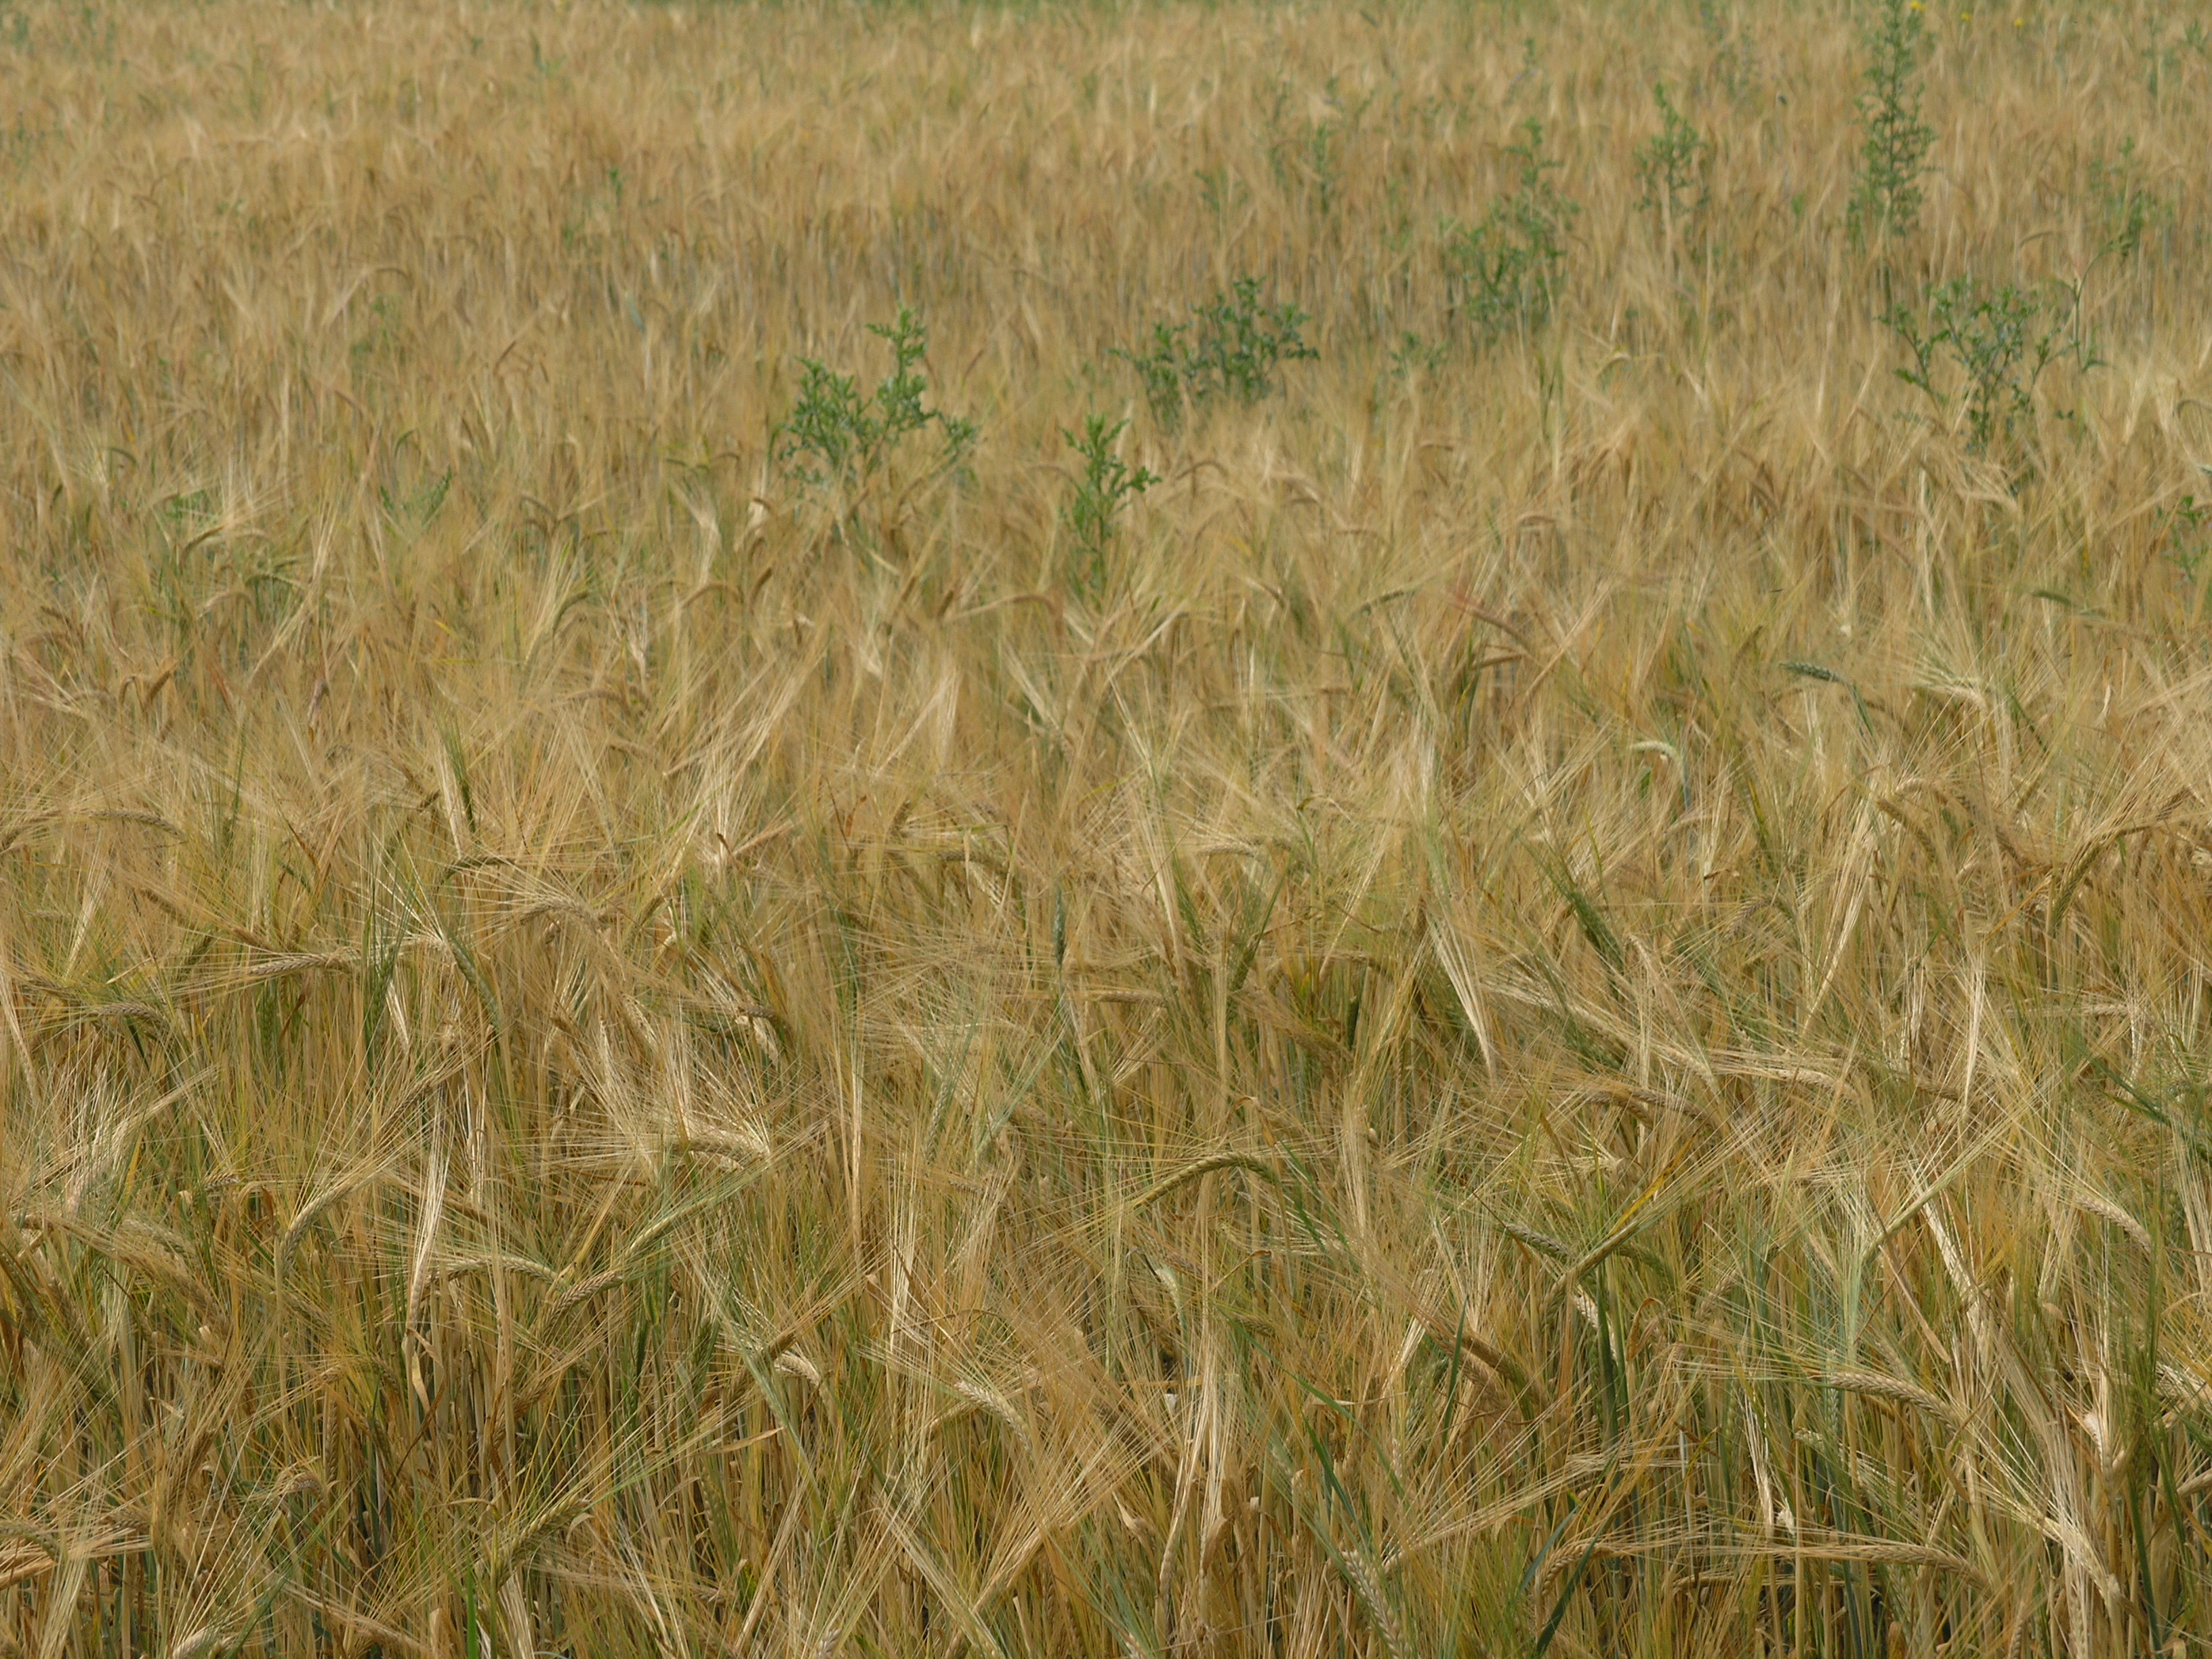
\includegraphics[width=\linewidth,height=\textheight,keepaspectratio]{/home/mkg/Dropbox/images/2005-07-09-a 100.jpg}
    \captionlistentry[figure]{\url{\protect\detokenize{}}}
\end{figure}

\KOMAoptions{pagesize}
\clearpage
\recalctypearea
\newpage
\noindent
Filename: None\\ 
Date taken: 2005:08:20 11:58:52\\ 
GPS longitude: None\\ 
GPS latitude: None\\ 
Make: OLYMPUS CORPORATION\\ 
Model: C8080WZ\\ 
Focal length (35mm eq): None\\ 
Exposure: 0.00625\\ 
F stop: 3.5\\ 
ISO: 50\\ 
Width: 3264\\ 
Height: 2448\\ 

\clearpage
\recalctypearea
\newpage
\noindent
\begin{figure}
    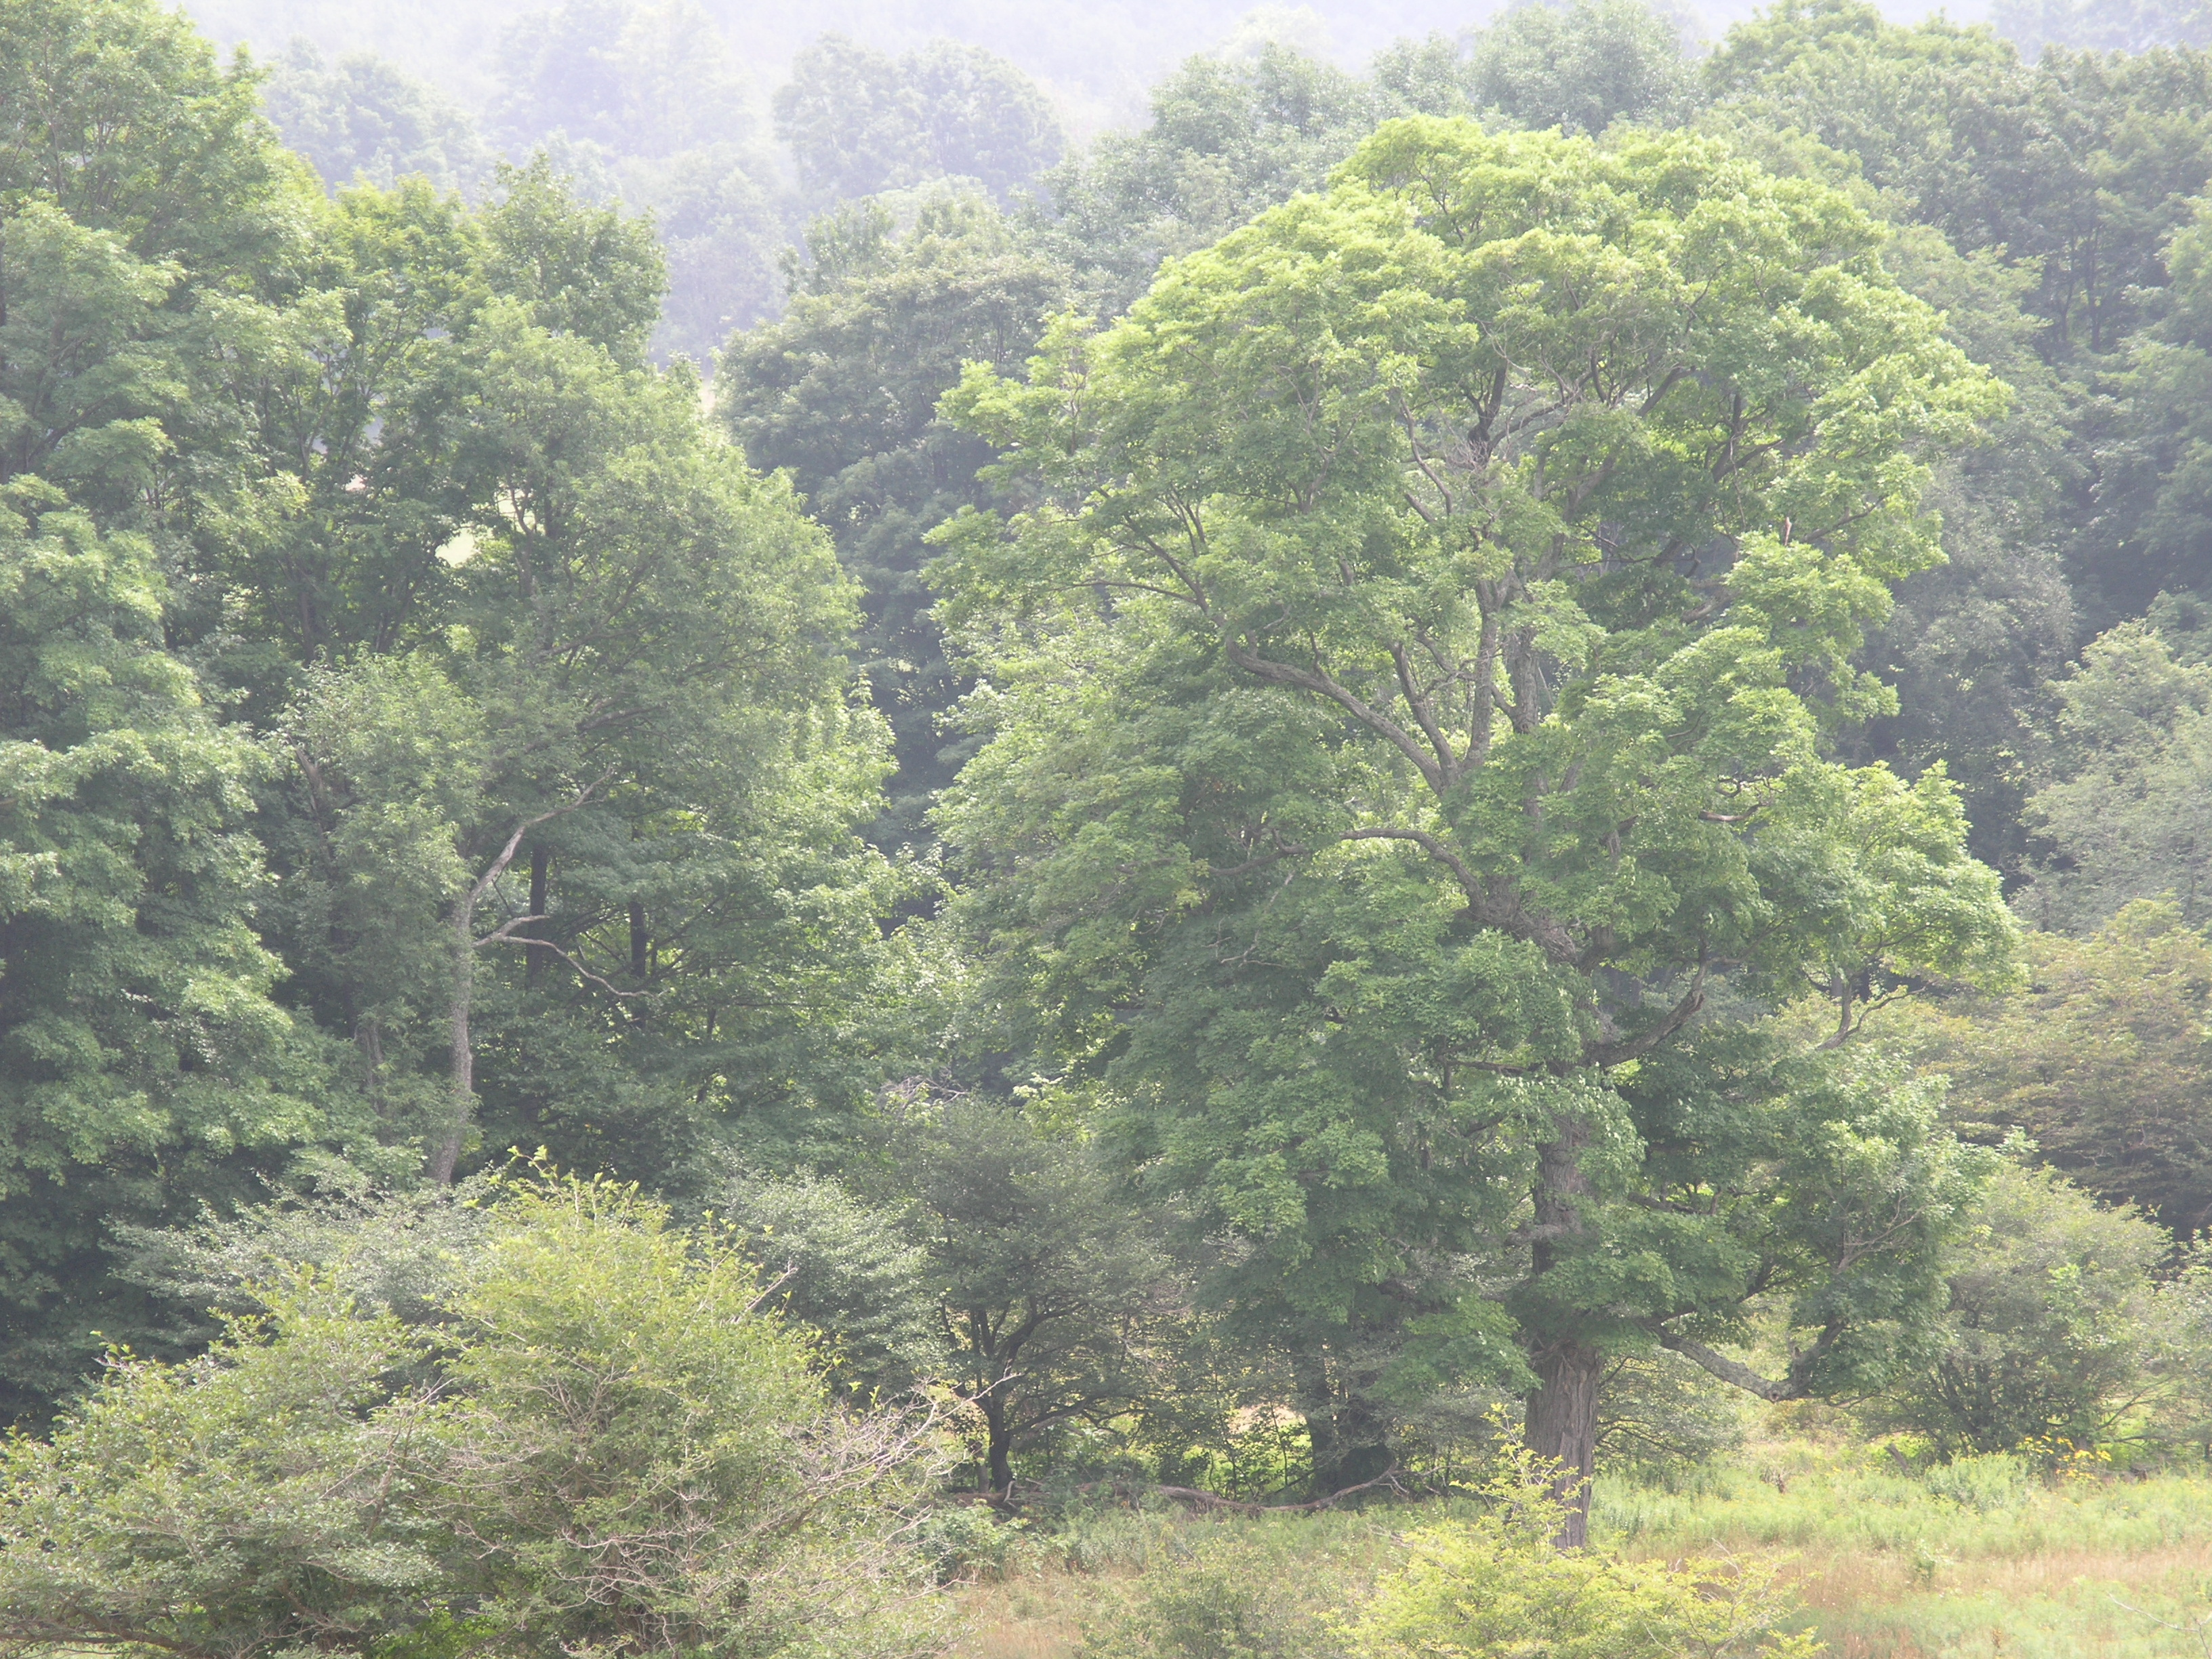
\includegraphics[width=\linewidth,height=\textheight,keepaspectratio]{/home/mkg/Dropbox/images/2005-10-02-a 020.jpg}
    \captionlistentry[figure]{\url{\protect\detokenize{}}}
\end{figure}

\KOMAoptions{pagesize}
\clearpage
\recalctypearea
\newpage
\noindent
Filename: None\\ 
Date taken: 2005:10:10 08:58:44\\ 
GPS longitude: None\\ 
GPS latitude: None\\ 
Make: OLYMPUS CORPORATION\\ 
Model: C8080WZ\\ 
Focal length (35mm eq): None\\ 
Exposure: 0.004\\ 
F stop: 3.5\\ 
ISO: 50\\ 
Width: 3264\\ 
Height: 2448\\ 

\clearpage
\recalctypearea
\newpage
\noindent
\begin{figure}
    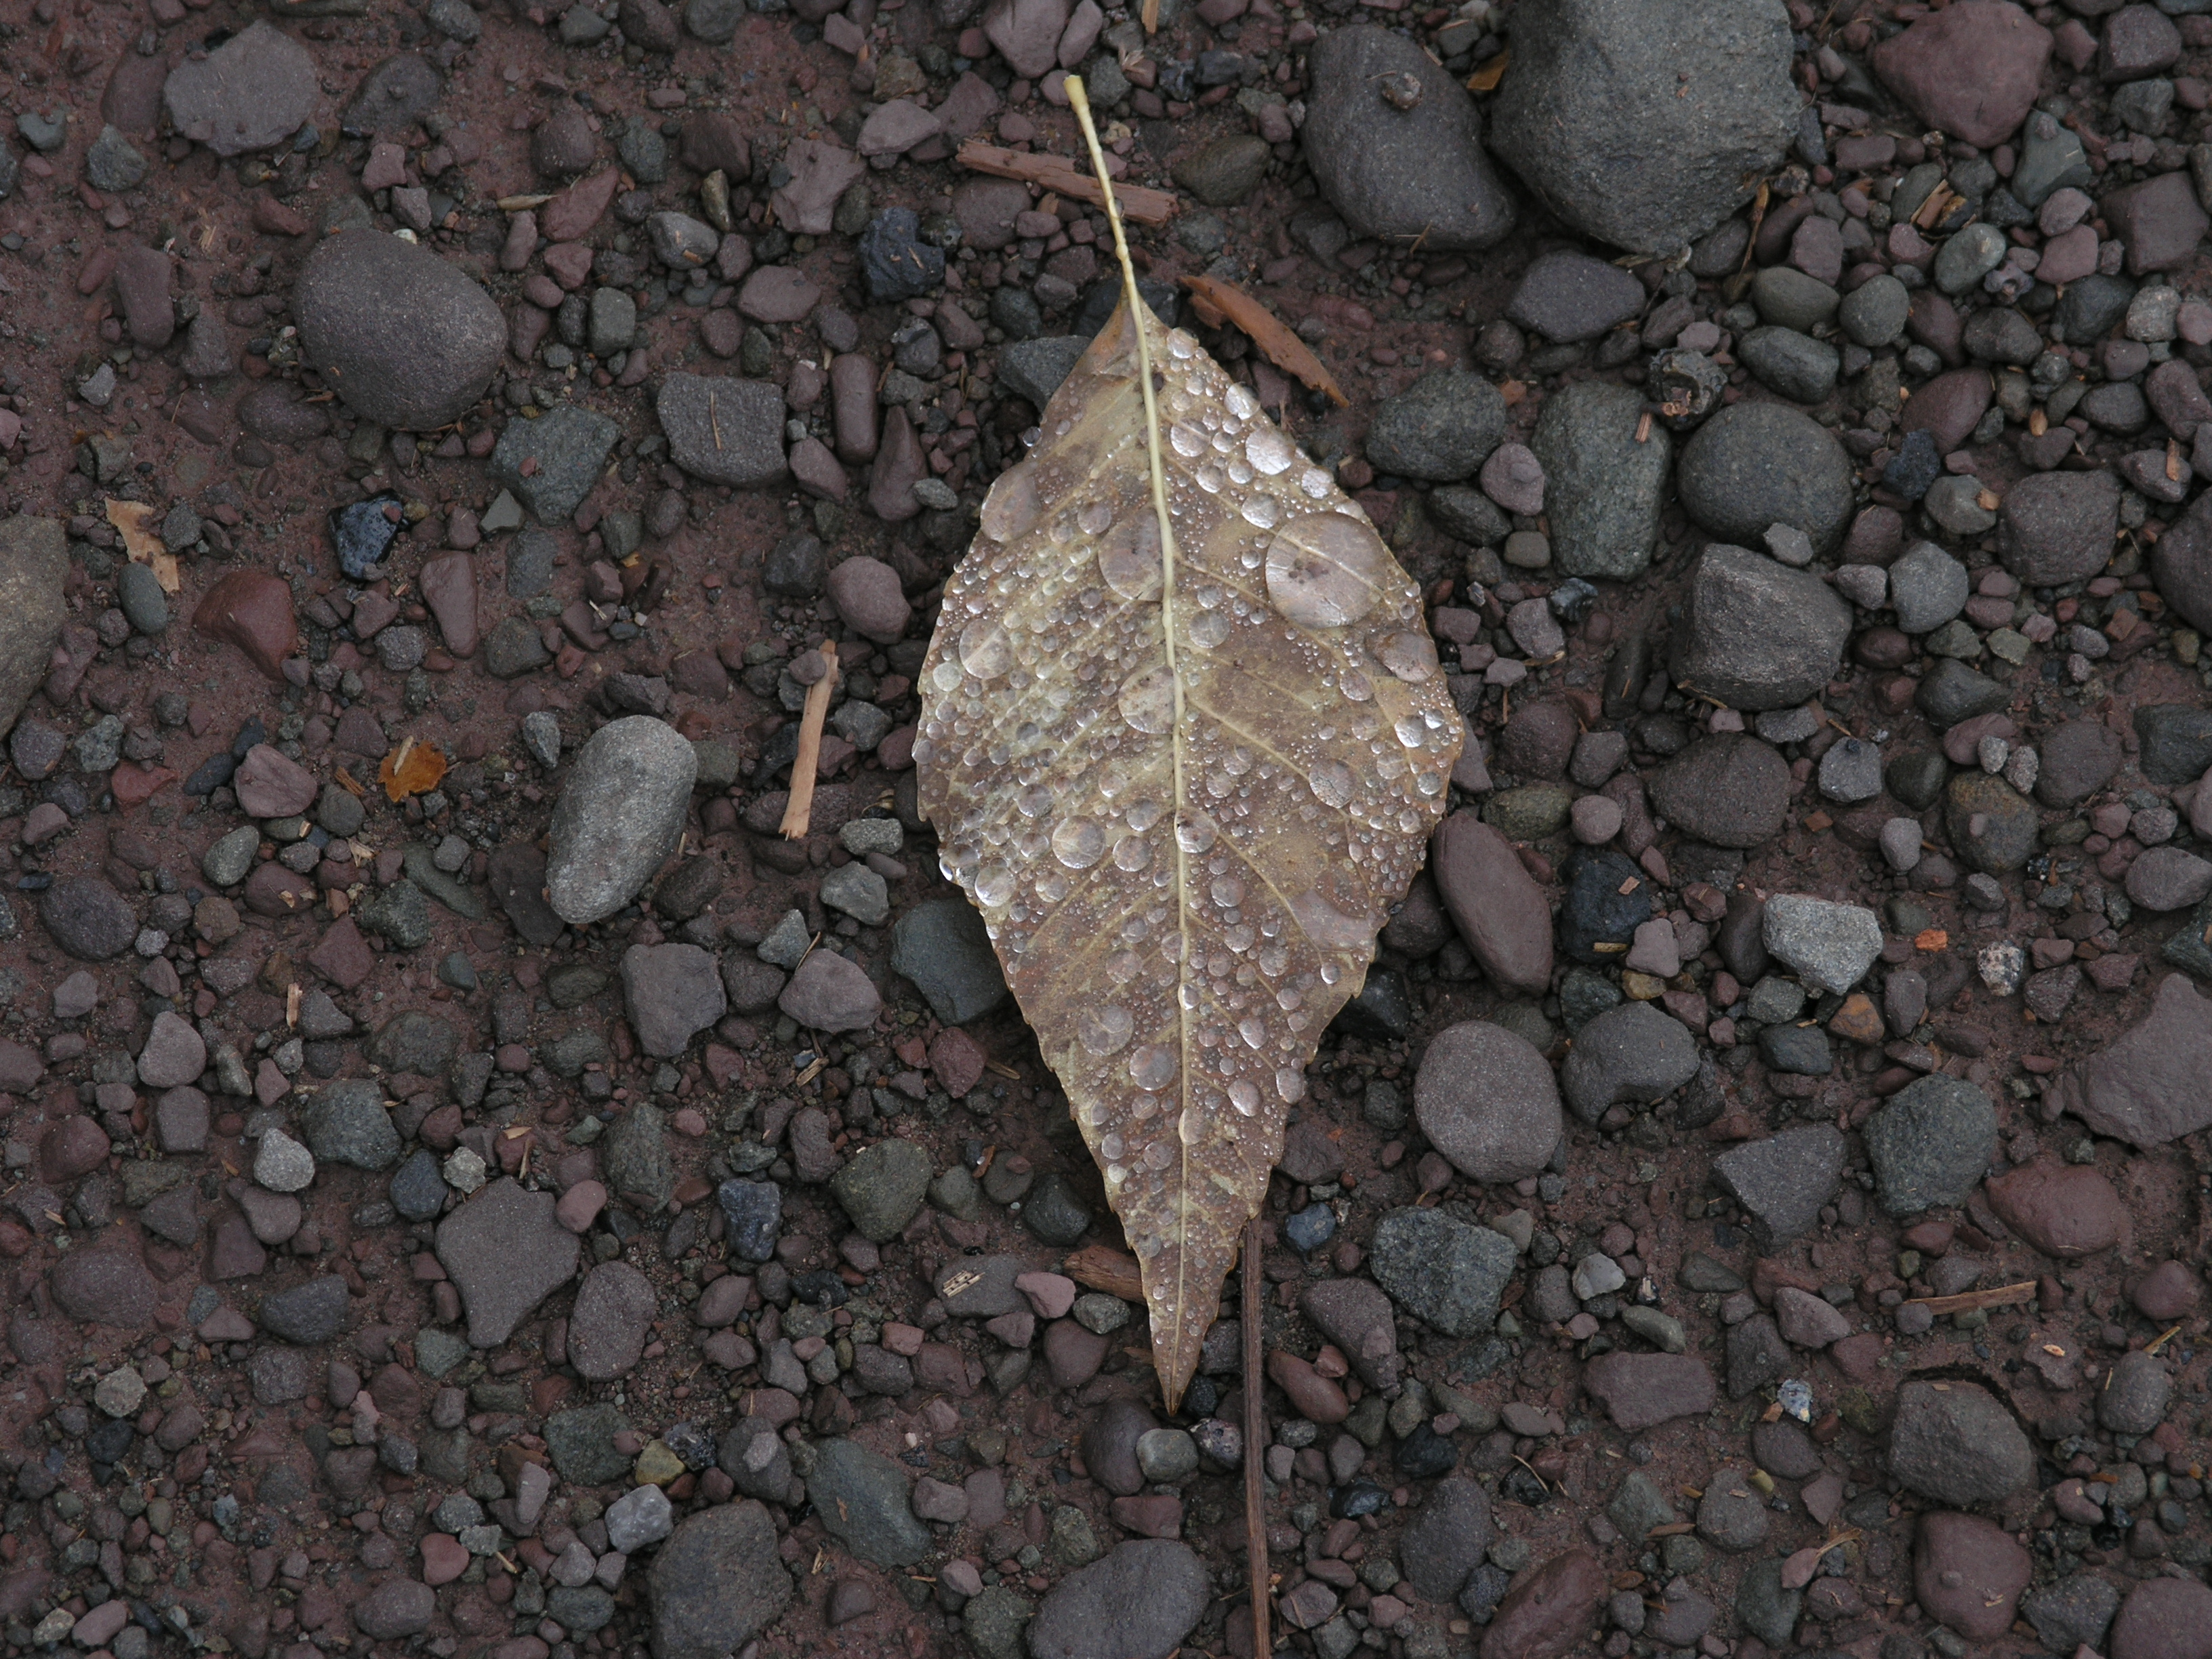
\includegraphics[width=\linewidth,height=\textheight,keepaspectratio]{/home/mkg/Dropbox/images/2005-10-10a 053.jpg}
    \captionlistentry[figure]{\url{\protect\detokenize{An old tree on our farm in Bovina, New York.}}}
\end{figure}

\KOMAoptions{pagesize}
\clearpage
\recalctypearea
\newpage
\noindent
Filename: None\\ 
Date taken: 2009:08:16 18:56:43\\ 
GPS longitude: None\\ 
GPS latitude: None\\ 
Make: Canon\\ 
Model: Canon PowerShot G7\\ 
Focal length (35mm eq): None\\ 
Exposure: 0.005\\ 
F stop: 4.0\\ 
ISO: None\\ 
Width: 3648\\ 
Height: 2736\\ 

\clearpage
\recalctypearea
\newpage
\noindent
\begin{figure}
    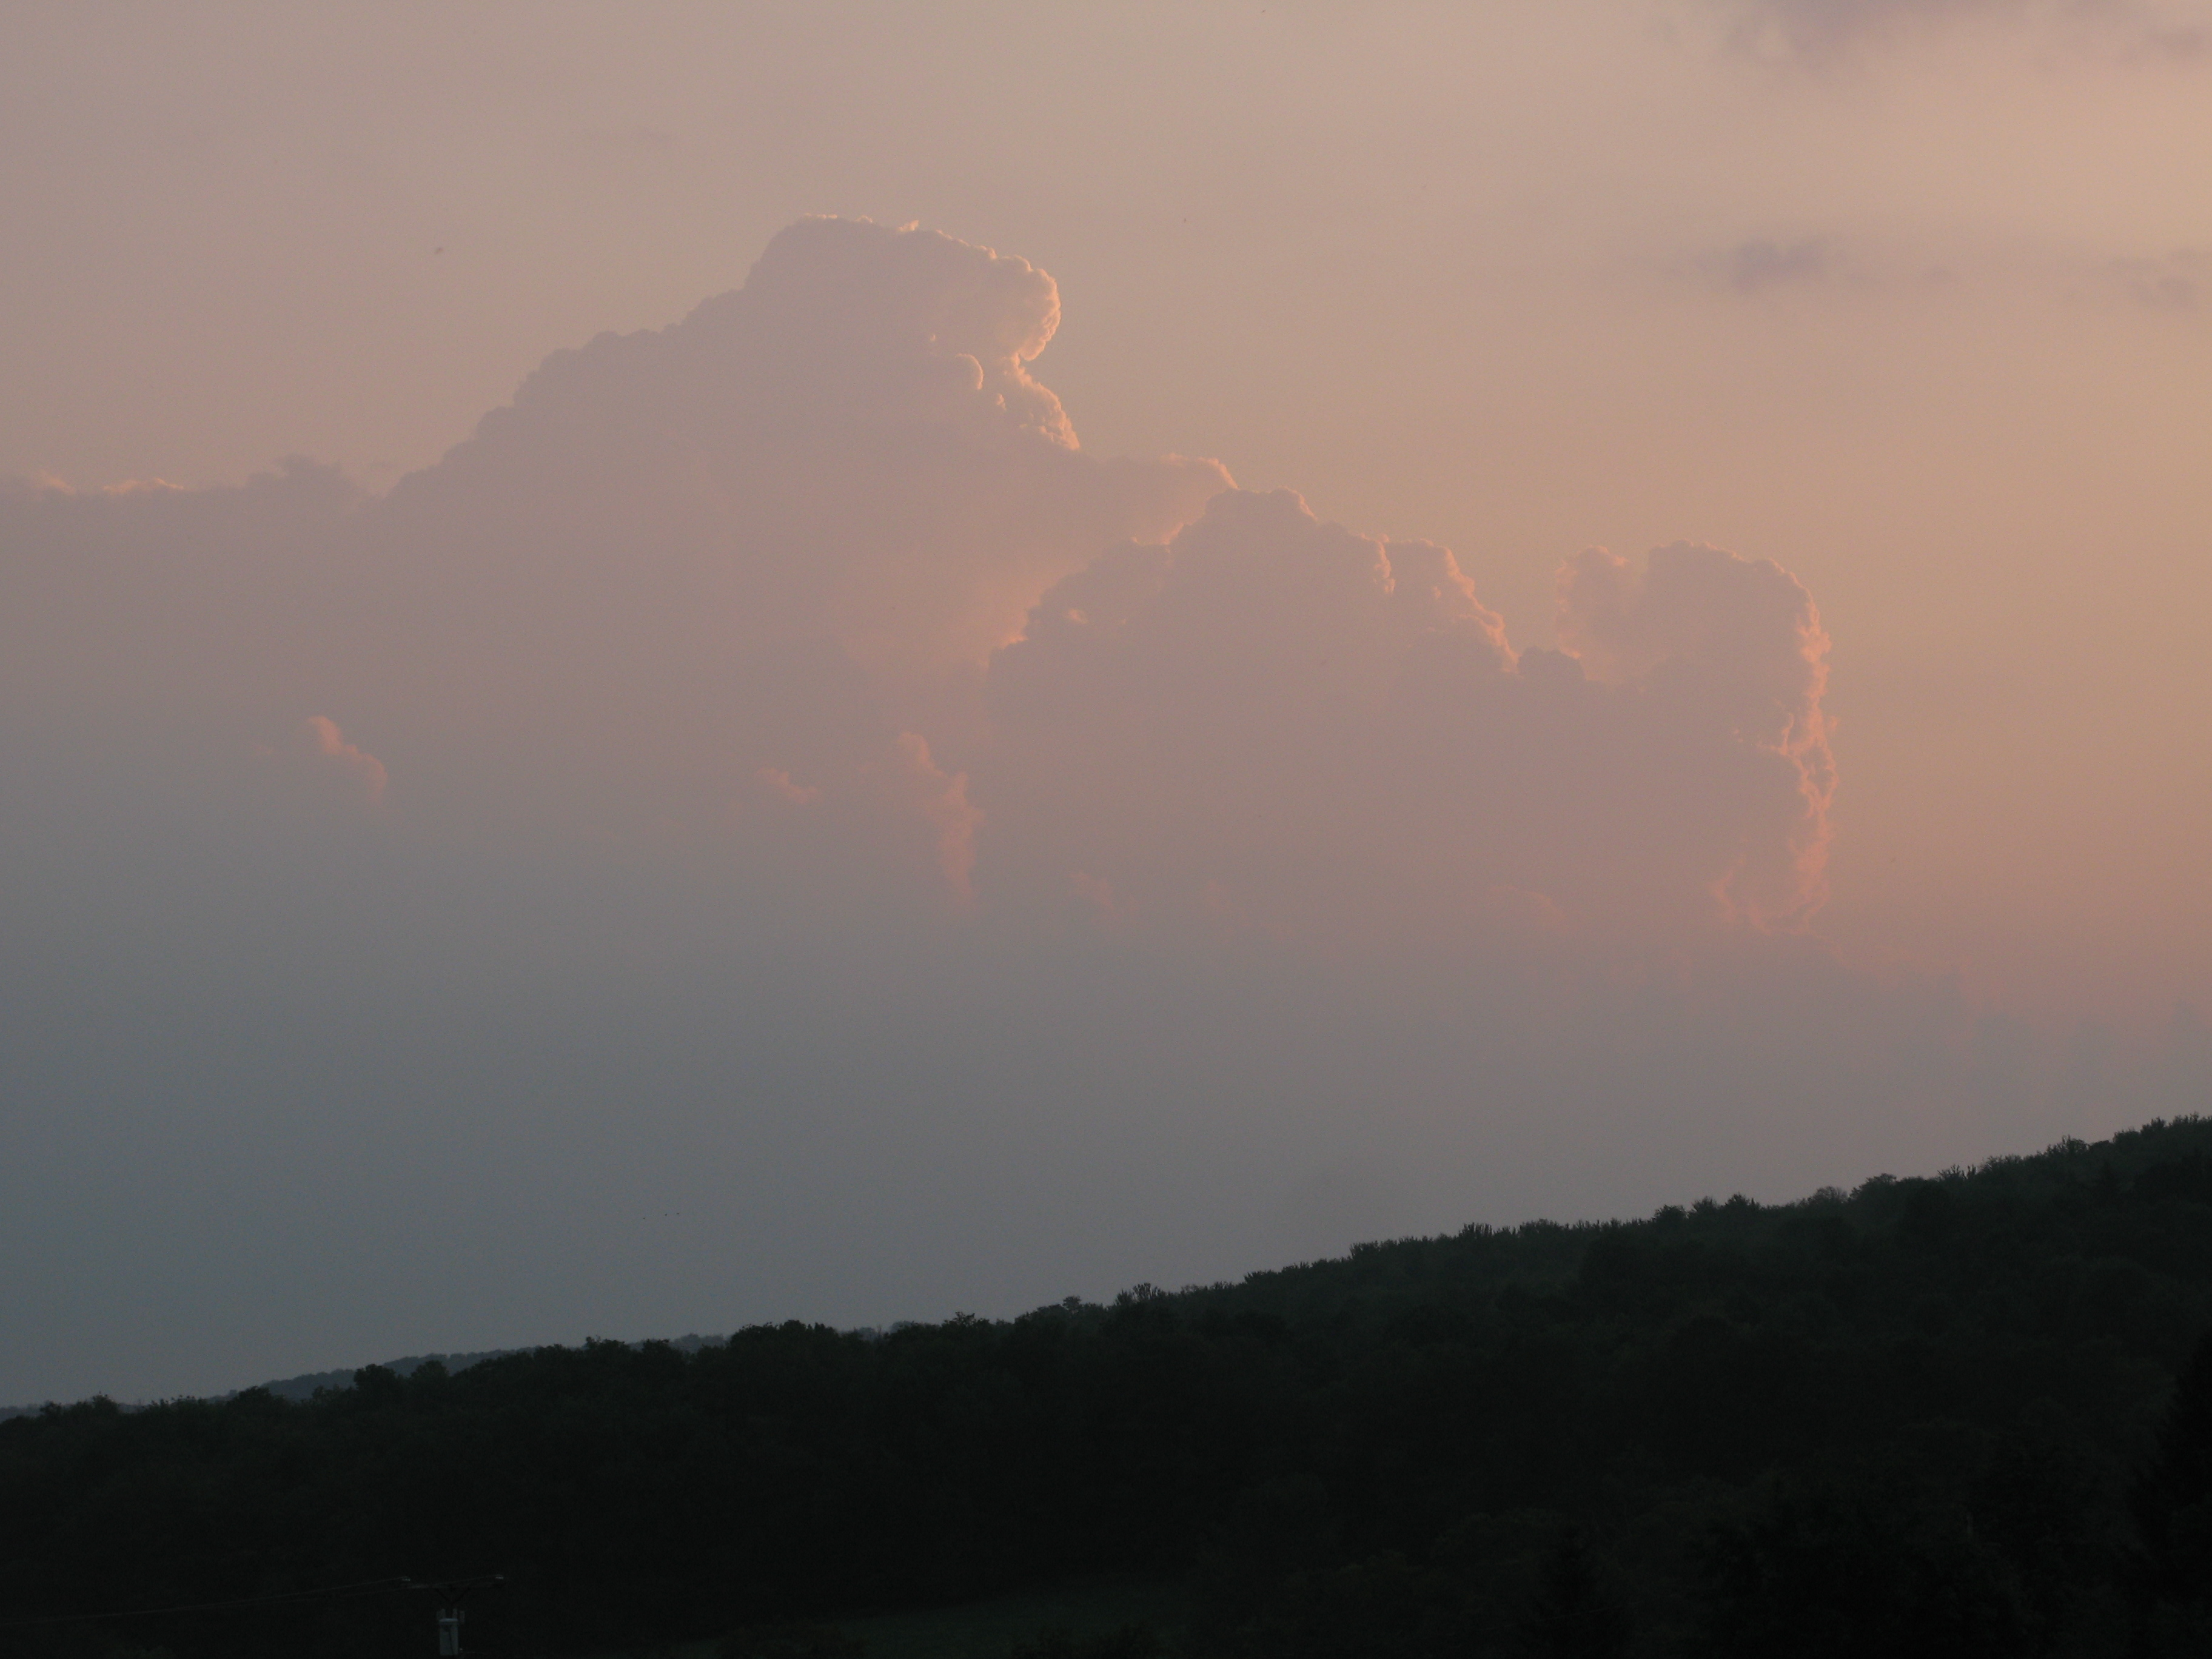
\includegraphics[width=\linewidth,height=\textheight,keepaspectratio]{/home/mkg/Dropbox/images/2009-08-27-a 097.jpg}
    \captionlistentry[figure]{\url{\protect\detokenize{}}}
\end{figure}

\KOMAoptions{pagesize}
\clearpage
\recalctypearea
\newpage
\noindent
Filename: None\\ 
Date taken: 2013:04:01 06:21:41\\ 
GPS longitude: None\\ 
GPS latitude: None\\ 
Make: SONY\\ 
Model: DSC-RX100\\ 
Focal length (35mm eq): 44\\ 
Exposure: 0.01\\ 
F stop: 3.5\\ 
ISO: 125\\ 
Width: 5472\\ 
Height: 3648\\ 

\clearpage
\recalctypearea
\newpage
\noindent
\begin{figure}
    \includegraphics[width=\linewidth,height=\textheight,keepaspectratio]{/home/mkg/Dropbox/images/DSC01131.JPG}
    \captionlistentry[figure]{\url{\protect\detokenize{}}}
\end{figure}

\KOMAoptions{pagesize}
\clearpage
\recalctypearea
\newpage
\noindent
Filename: None\\ 
Date taken: 2013:04:06 18:06:00\\ 
GPS longitude: None\\ 
GPS latitude: None\\ 
Make: SONY\\ 
Model: DSC-RX100\\ 
Focal length (35mm eq): 54\\ 
Exposure: 0.01\\ 
F stop: 4.5\\ 
ISO: 125\\ 
Width: 5472\\ 
Height: 3648\\ 

\clearpage
\recalctypearea
\newpage
\noindent
\begin{figure}
    \includegraphics[width=\linewidth,height=\textheight,keepaspectratio]{/home/mkg/Dropbox/images/DSC01240.JPG}
    \captionlistentry[figure]{\url{\protect\detokenize{}}}
\end{figure}

\KOMAoptions{pagesize}
\clearpage
\recalctypearea
\newpage
\noindent
Filename: None\\ 
Date taken: 2013:08:25 19:38:23\\ 
GPS longitude: None\\ 
GPS latitude: None\\ 
Make: SONY\\ 
Model: DSC-RX100\\ 
Focal length (35mm eq): 100\\ 
Exposure: 0.01\\ 
F stop: 4.9\\ 
ISO: 800\\ 
Width: 5472\\ 
Height: 3648\\ 

\clearpage
\recalctypearea
\newpage
\noindent
\begin{figure}
    \includegraphics[width=\linewidth,height=\textheight,keepaspectratio]{/home/mkg/Dropbox/images/DSC01577.JPG}
    \captionlistentry[figure]{\url{\protect\detokenize{The old ice cream stand in Stamford, New York. Replaced by a newer (but not quite as friendly and funky) version.}}}
\end{figure}

\KOMAoptions{pagesize}
\clearpage
\recalctypearea
\newpage
\noindent
Filename: None\\ 
Date taken: 2013:10:25 10:07:59\\ 
GPS longitude: None\\ 
GPS latitude: None\\ 
Make: SONY\\ 
Model: DSC-RX100\\ 
Focal length (35mm eq): 46\\ 
Exposure: 0.02\\ 
F stop: 3.2\\ 
ISO: 3200\\ 
Width: 5368\\ 
Height: 3484\\ 

\clearpage
\recalctypearea
\newpage
\noindent
\begin{figure}
    \includegraphics[width=\linewidth,height=\textheight,keepaspectratio]{/home/mkg/Dropbox/images/DSC01723.JPG}
    \captionlistentry[figure]{\url{\protect\detokenize{Computer music luminaries Richard Boulanger (left) and Jean-Claude Risset, and their spouses, at the 2nd International Csound Conference, Berklee School of Music, Boston.}}}
\end{figure}

\KOMAoptions{pagesize}
\clearpage
\recalctypearea
\newpage
\noindent
Filename: None\\ 
Date taken: 2013:12:06 07:04:13\\ 
GPS longitude: None\\ 
GPS latitude: None\\ 
Make: SONY\\ 
Model: DSC-RX100\\ 
Focal length (35mm eq): 78\\ 
Exposure: 0.002\\ 
F stop: 5.6\\ 
ISO: 125\\ 
Width: 5472\\ 
Height: 3648\\ 

\clearpage
\recalctypearea
\newpage
\noindent
\begin{figure}
    \includegraphics[width=\linewidth,height=\textheight,keepaspectratio]{/home/mkg/Dropbox/images/DSC02503.JPG}
    \captionlistentry[figure]{\url{\protect\detokenize{Magazine covers, Girona, Spain.}}}
\end{figure}

\KOMAoptions{pagesize}
\clearpage
\recalctypearea
\newpage
\noindent
Filename: None\\ 
Date taken: 2013:12:08 09:24:07\\ 
GPS longitude: None\\ 
GPS latitude: None\\ 
Make: SONY\\ 
Model: DSC-RX100\\ 
Focal length (35mm eq): 100\\ 
Exposure: 0.005\\ 
F stop: 5.6\\ 
ISO: 125\\ 
Width: 5472\\ 
Height: 3648\\ 

\clearpage
\recalctypearea
\newpage
\noindent
\begin{figure}
    \includegraphics[width=\linewidth,height=\textheight,keepaspectratio]{/home/mkg/Dropbox/images/DSC02654.JPG}
    \captionlistentry[figure]{\url{\protect\detokenize{}}}
\end{figure}

\KOMAoptions{pagesize}
\clearpage
\recalctypearea
\newpage
\noindent
Filename: None\\ 
Date taken: 2019:03:09 22:01:42\\ 
GPS longitude: None\\ 
GPS latitude: None\\ 
Make: SONY\\ 
Model: DSC-RX100M5\\ 
Focal length (35mm eq): 70\\ 
Exposure: 0.0125\\ 
F stop: 5.6\\ 
ISO: 125\\ 
Width: 5472\\ 
Height: 3648\\ 

\clearpage
\recalctypearea
\newpage
\noindent
\begin{figure}
    \includegraphics[width=\linewidth,height=\textheight,keepaspectratio]{/home/mkg/Dropbox/images/RX100M5/100MSDCF/DSC06075.JPG}
    \captionlistentry[figure]{\url{\protect\detokenize{}}}
\end{figure}

\KOMAoptions{pagesize}
\clearpage
\recalctypearea
\newpage
\noindent
Filename: None\\ 
Date taken: 2019:03:29 15:46:37\\ 
GPS longitude: None\\ 
GPS latitude: None\\ 
Make: SONY\\ 
Model: DSC-RX100M5\\ 
Focal length (35mm eq): 24\\ 
Exposure: 0.00625\\ 
F stop: 4.0\\ 
ISO: 125\\ 
Width: 5472\\ 
Height: 3648\\ 

\clearpage
\recalctypearea
\newpage
\noindent
\begin{figure}
    \includegraphics[width=\linewidth,height=\textheight,keepaspectratio]{/home/mkg/Dropbox/images/RX100/100MSDCF/DSC06643.JPG}
    \captionlistentry[figure]{\url{\protect\detokenize{}}}
\end{figure}

\KOMAoptions{pagesize}
\clearpage
\recalctypearea
\newpage
\noindent
Filename: None\\ 
Date taken: 2019:03:26 22:40:10\\ 
GPS longitude: None\\ 
GPS latitude: None\\ 
Make: SONY\\ 
Model: DSC-RX100M5\\ 
Focal length (35mm eq): 70\\ 
Exposure: 0.0015625\\ 
F stop: 4.0\\ 
ISO: 125\\ 
Width: 5472\\ 
Height: 3648\\ 

\clearpage
\recalctypearea
\newpage
\noindent
\begin{figure}
    \includegraphics[width=\linewidth,height=\textheight,keepaspectratio]{/home/mkg/Dropbox/images/RX100M5/100MSDCF/DSC06552.JPG}
    \captionlistentry[figure]{\url{\protect\detokenize{Chinese Garden, Dunedin, New Zealand.}}}
\end{figure}

\KOMAoptions{pagesize}
\clearpage
\recalctypearea
\newpage
\noindent
Filename: None\\ 
Date taken: 2016:12:03 19:03:49\\ 
GPS longitude: None\\ 
GPS latitude: None\\ 
Make: SONY\\ 
Model: DSC-RX100\\ 
Focal length (35mm eq): 28\\ 
Exposure: 0.025\\ 
F stop: 1.8\\ 
ISO: 3200\\ 
Width: 5472\\ 
Height: 3648\\ 

\clearpage
\recalctypearea
\newpage
\noindent
\begin{figure}
    \includegraphics[width=\linewidth,height=\textheight,keepaspectratio]{/home/mkg/Dropbox/images/RX100/100MSDCF/DSC00956.JPG}
    \captionlistentry[figure]{\url{\protect\detokenize{Lower East Side, Manhattan.}}}
\end{figure}

\KOMAoptions{pagesize}
\clearpage
\recalctypearea
\newpage
\noindent
Filename: None\\ 
Date taken: 2013:12:11 10:47:13\\ 
GPS longitude: None\\ 
GPS latitude: None\\ 
Make: SONY\\ 
Model: DSC-RX100\\ 
Focal length (35mm eq): 57\\ 
Exposure: 0.06666666666666667\\ 
F stop: 3.5\\ 
ISO: 800\\ 
Width: 3476\\ 
Height: 5362\\ 

\clearpage
\recalctypearea
\newpage
\noindent
\begin{figure}
    \includegraphics[width=\linewidth,height=\textheight,keepaspectratio]{/home/mkg/Dropbox/images/DSC02857.JPG}
    \captionlistentry[figure]{\url{\protect\detokenize{The Father offering the Son, Narbonne, France.}}}
\end{figure}

\KOMAoptions{pagesize}
\clearpage
\recalctypearea
\newpage
\noindent
Filename: None\\ 
Date taken: 2013:12:11 13:36:30\\ 
GPS longitude: None\\ 
GPS latitude: None\\ 
Make: SONY\\ 
Model: DSC-RX100\\ 
Focal length (35mm eq): 72\\ 
Exposure: 0.0125\\ 
F stop: 4.0\\ 
ISO: 3200\\ 
Width: 5376\\ 
Height: 3500\\ 

\clearpage
\recalctypearea
\newpage
\noindent
\begin{figure}
    \includegraphics[width=\linewidth,height=\textheight,keepaspectratio]{/home/mkg/Dropbox/images/DSC02910.JPG}
    \captionlistentry[figure]{\url{\protect\detokenize{Christmas carnival in Carcassone, France.}}}
\end{figure}

\KOMAoptions{pagesize}
\clearpage
\recalctypearea
\newpage
\noindent
Filename: None\\ 
Date taken: 2016:04:06 13:12:31\\ 
GPS longitude: None\\ 
GPS latitude: None\\ 
Make: SONY\\ 
Model: DSC-RX100\\ 
Focal length (35mm eq): 28\\ 
Exposure: 0.03333333333333333\\ 
F stop: 1.8\\ 
ISO: 800\\ 
Width: 5470\\ 
Height: 3644\\ 

\clearpage
\recalctypearea
\newpage
\noindent
\begin{figure}
    \includegraphics[width=\linewidth,height=\textheight,keepaspectratio]{/home/mkg/Dropbox/images/DSC09755.JPG}
    \captionlistentry[figure]{\url{\protect\detokenize{Merry-go-round on the boardwalk in Tel Aviv, Israel.}}}
\end{figure}

\KOMAoptions{pagesize}
\clearpage
\recalctypearea
\newpage
\noindent
Filename: None\\ 
Date taken: 2013:06:04 13:43:30\\ 
GPS longitude: None\\ 
GPS latitude: None\\ 
Make: SAMSUNG\\ 
Model: SGH-M919\\ 
Focal length (35mm eq): 31\\ 
Exposure: 0.002506265664160401\\ 
F stop: 2.2\\ 
ISO: 50\\ 
Width: 4128\\ 
Height: 2322\\ 

\clearpage
\recalctypearea
\newpage
\noindent
\begin{figure}
    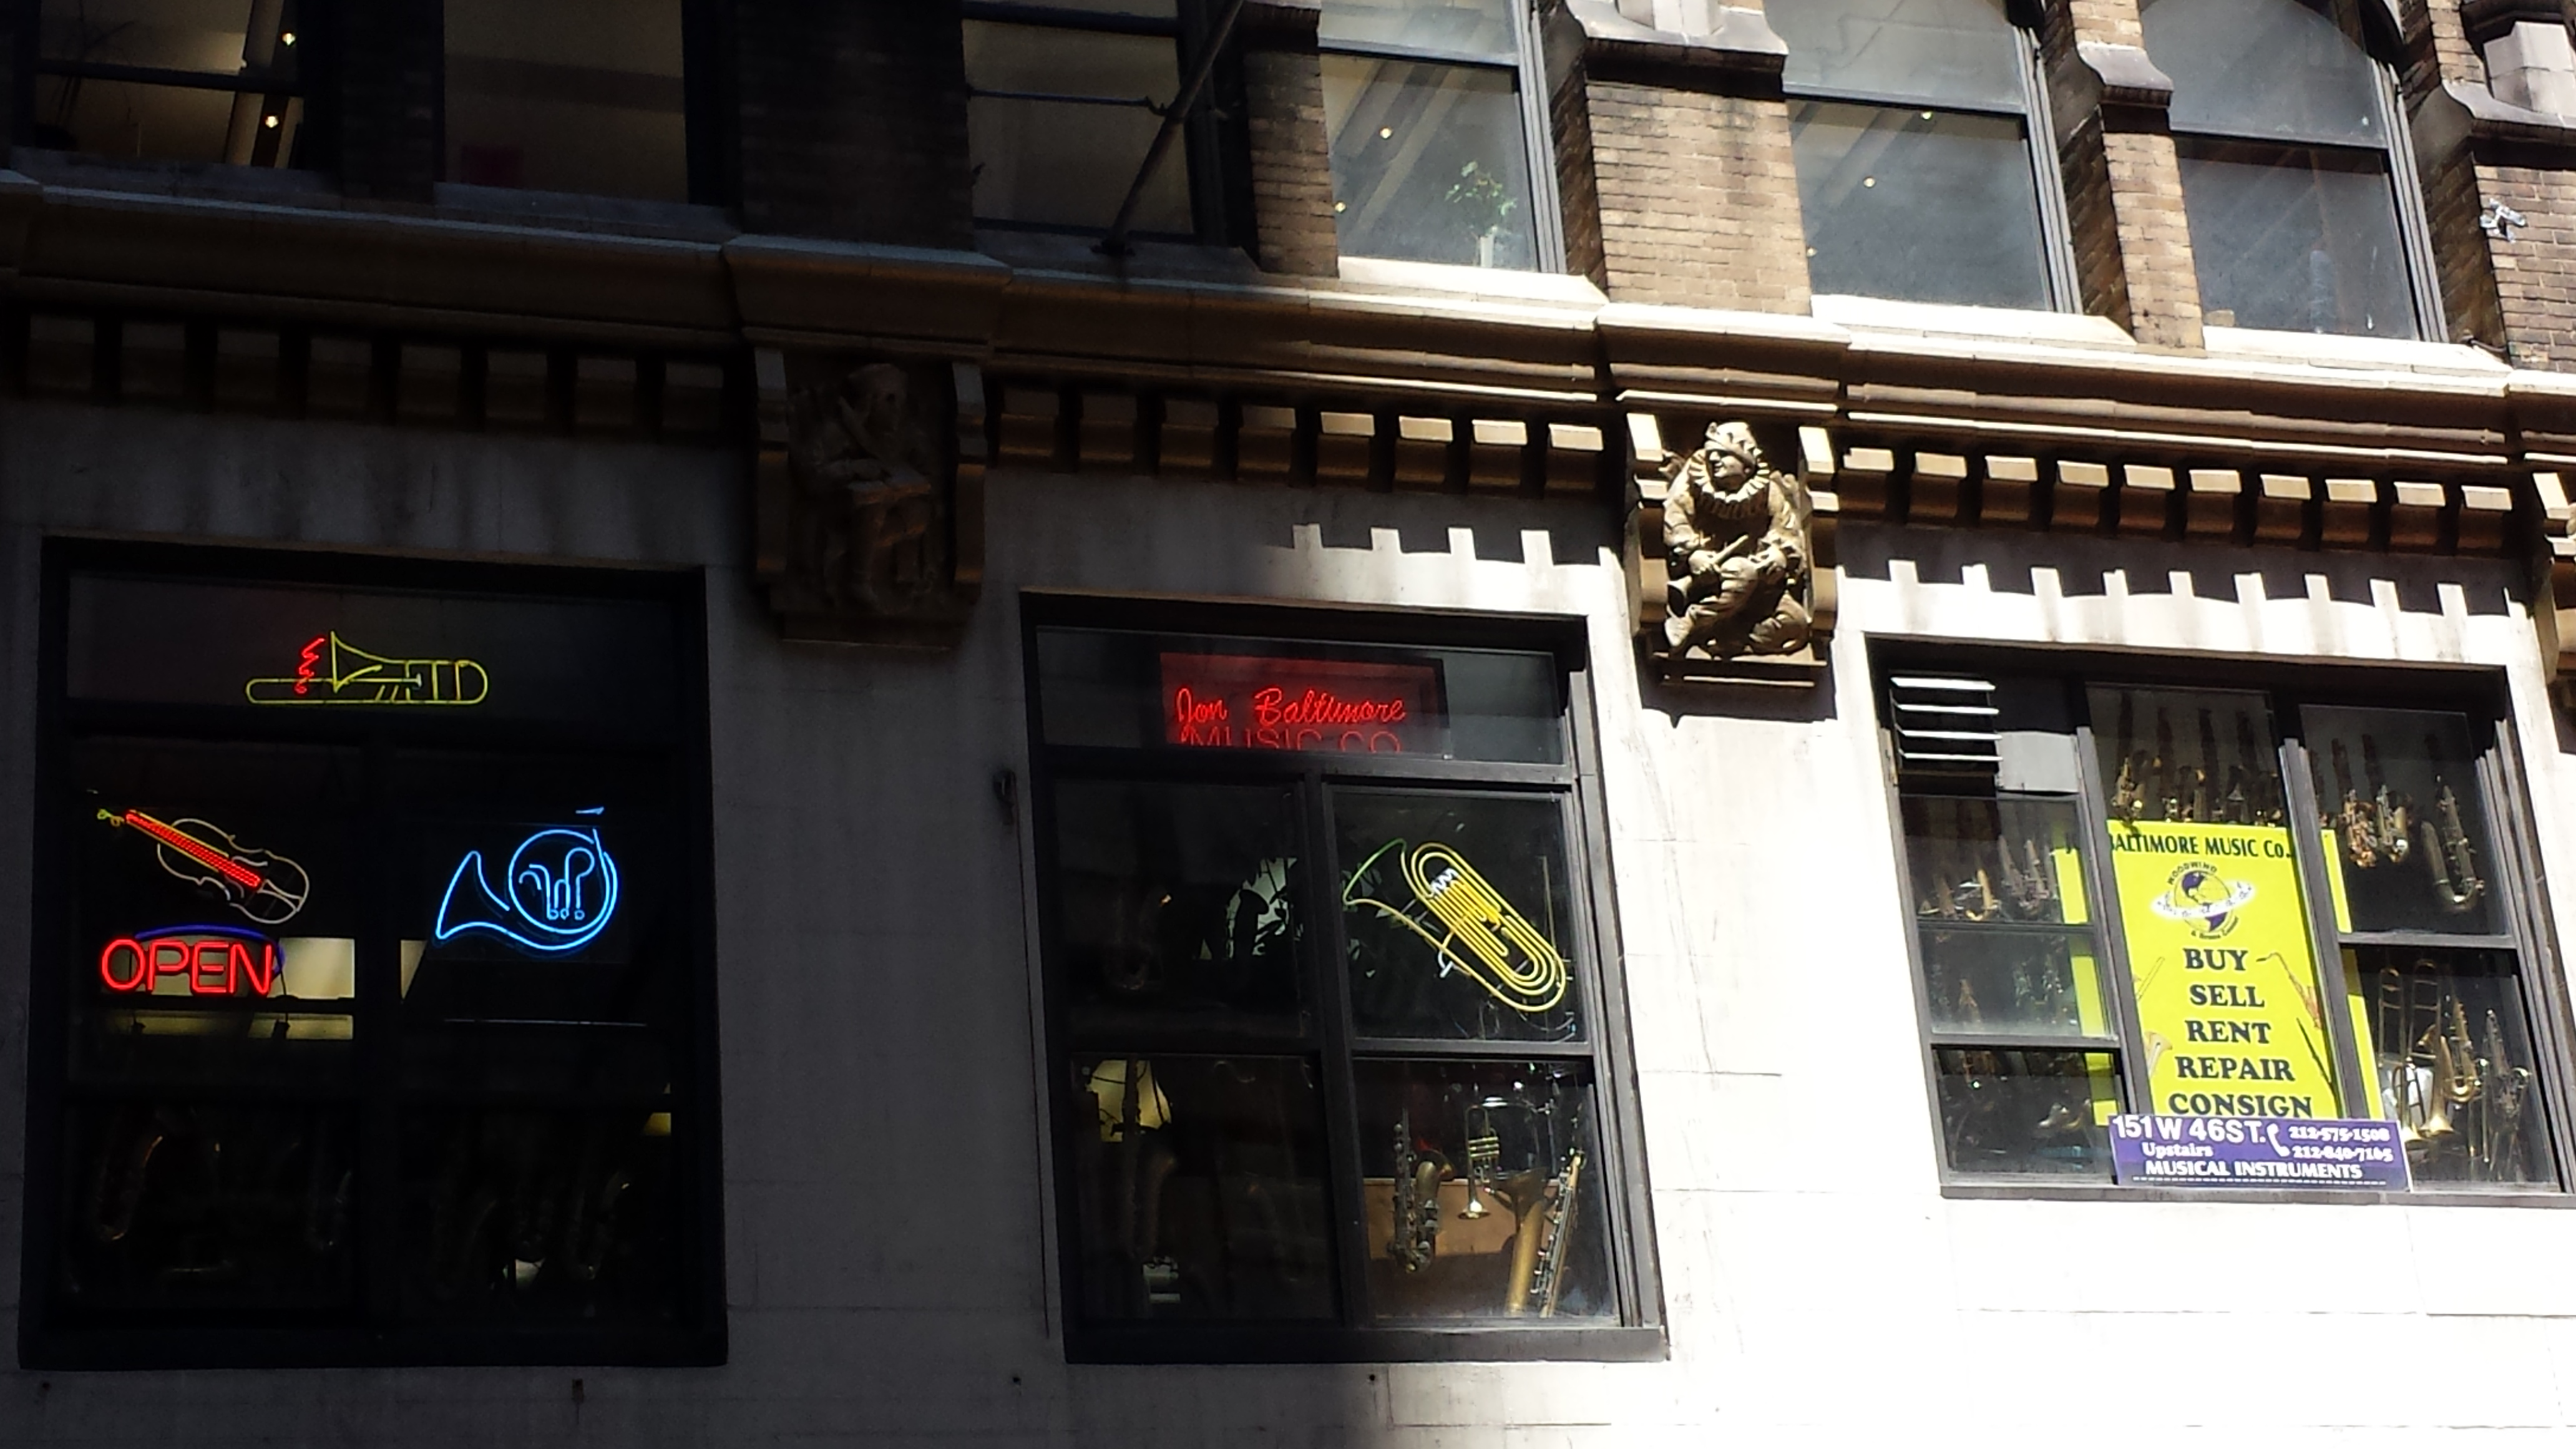
\includegraphics[width=\linewidth,height=\textheight,keepaspectratio]{/home/mkg/Dropbox/images/20130604_134331.jpg}
    \captionlistentry[figure]{\url{\protect\detokenize{A remnant of Music Row in Manhattan.}}}
\end{figure}

\KOMAoptions{pagesize}
\clearpage
\recalctypearea
\newpage
\noindent
Filename: None\\ 
Date taken: 2013:06:19 22:01:54\\ 
GPS longitude: None\\ 
GPS latitude: None\\ 
Make: SAMSUNG\\ 
Model: SGH-M919\\ 
Focal length (35mm eq): 31\\ 
Exposure: 0.004273504273504274\\ 
F stop: 2.2\\ 
ISO: 50\\ 
Width: 4128\\ 
Height: 2322\\ 

\clearpage
\recalctypearea
\newpage
\noindent
\begin{figure}
    \includegraphics[width=\linewidth,height=\textheight,keepaspectratio]{/home/mkg/Dropbox/images/20130619_080155.jpg}
    \captionlistentry[figure]{\url{\protect\detokenize{Central Park, Manhattan.}}}
\end{figure}

\KOMAoptions{pagesize}
\clearpage
\recalctypearea
\newpage
\noindent
Filename: None\\ 
Date taken: None\\ 
GPS longitude: None\\ 
GPS latitude: None\\ 
Make: \\ 
Model: \\ 
Focal length (35mm eq): None\\ 
Exposure: None\\ 
F stop: None\\ 
ISO: ()\\ 
Width: 2147\\ 
Height: 3186\\ 

\clearpage
\recalctypearea
\newpage
\noindent
\begin{figure}
    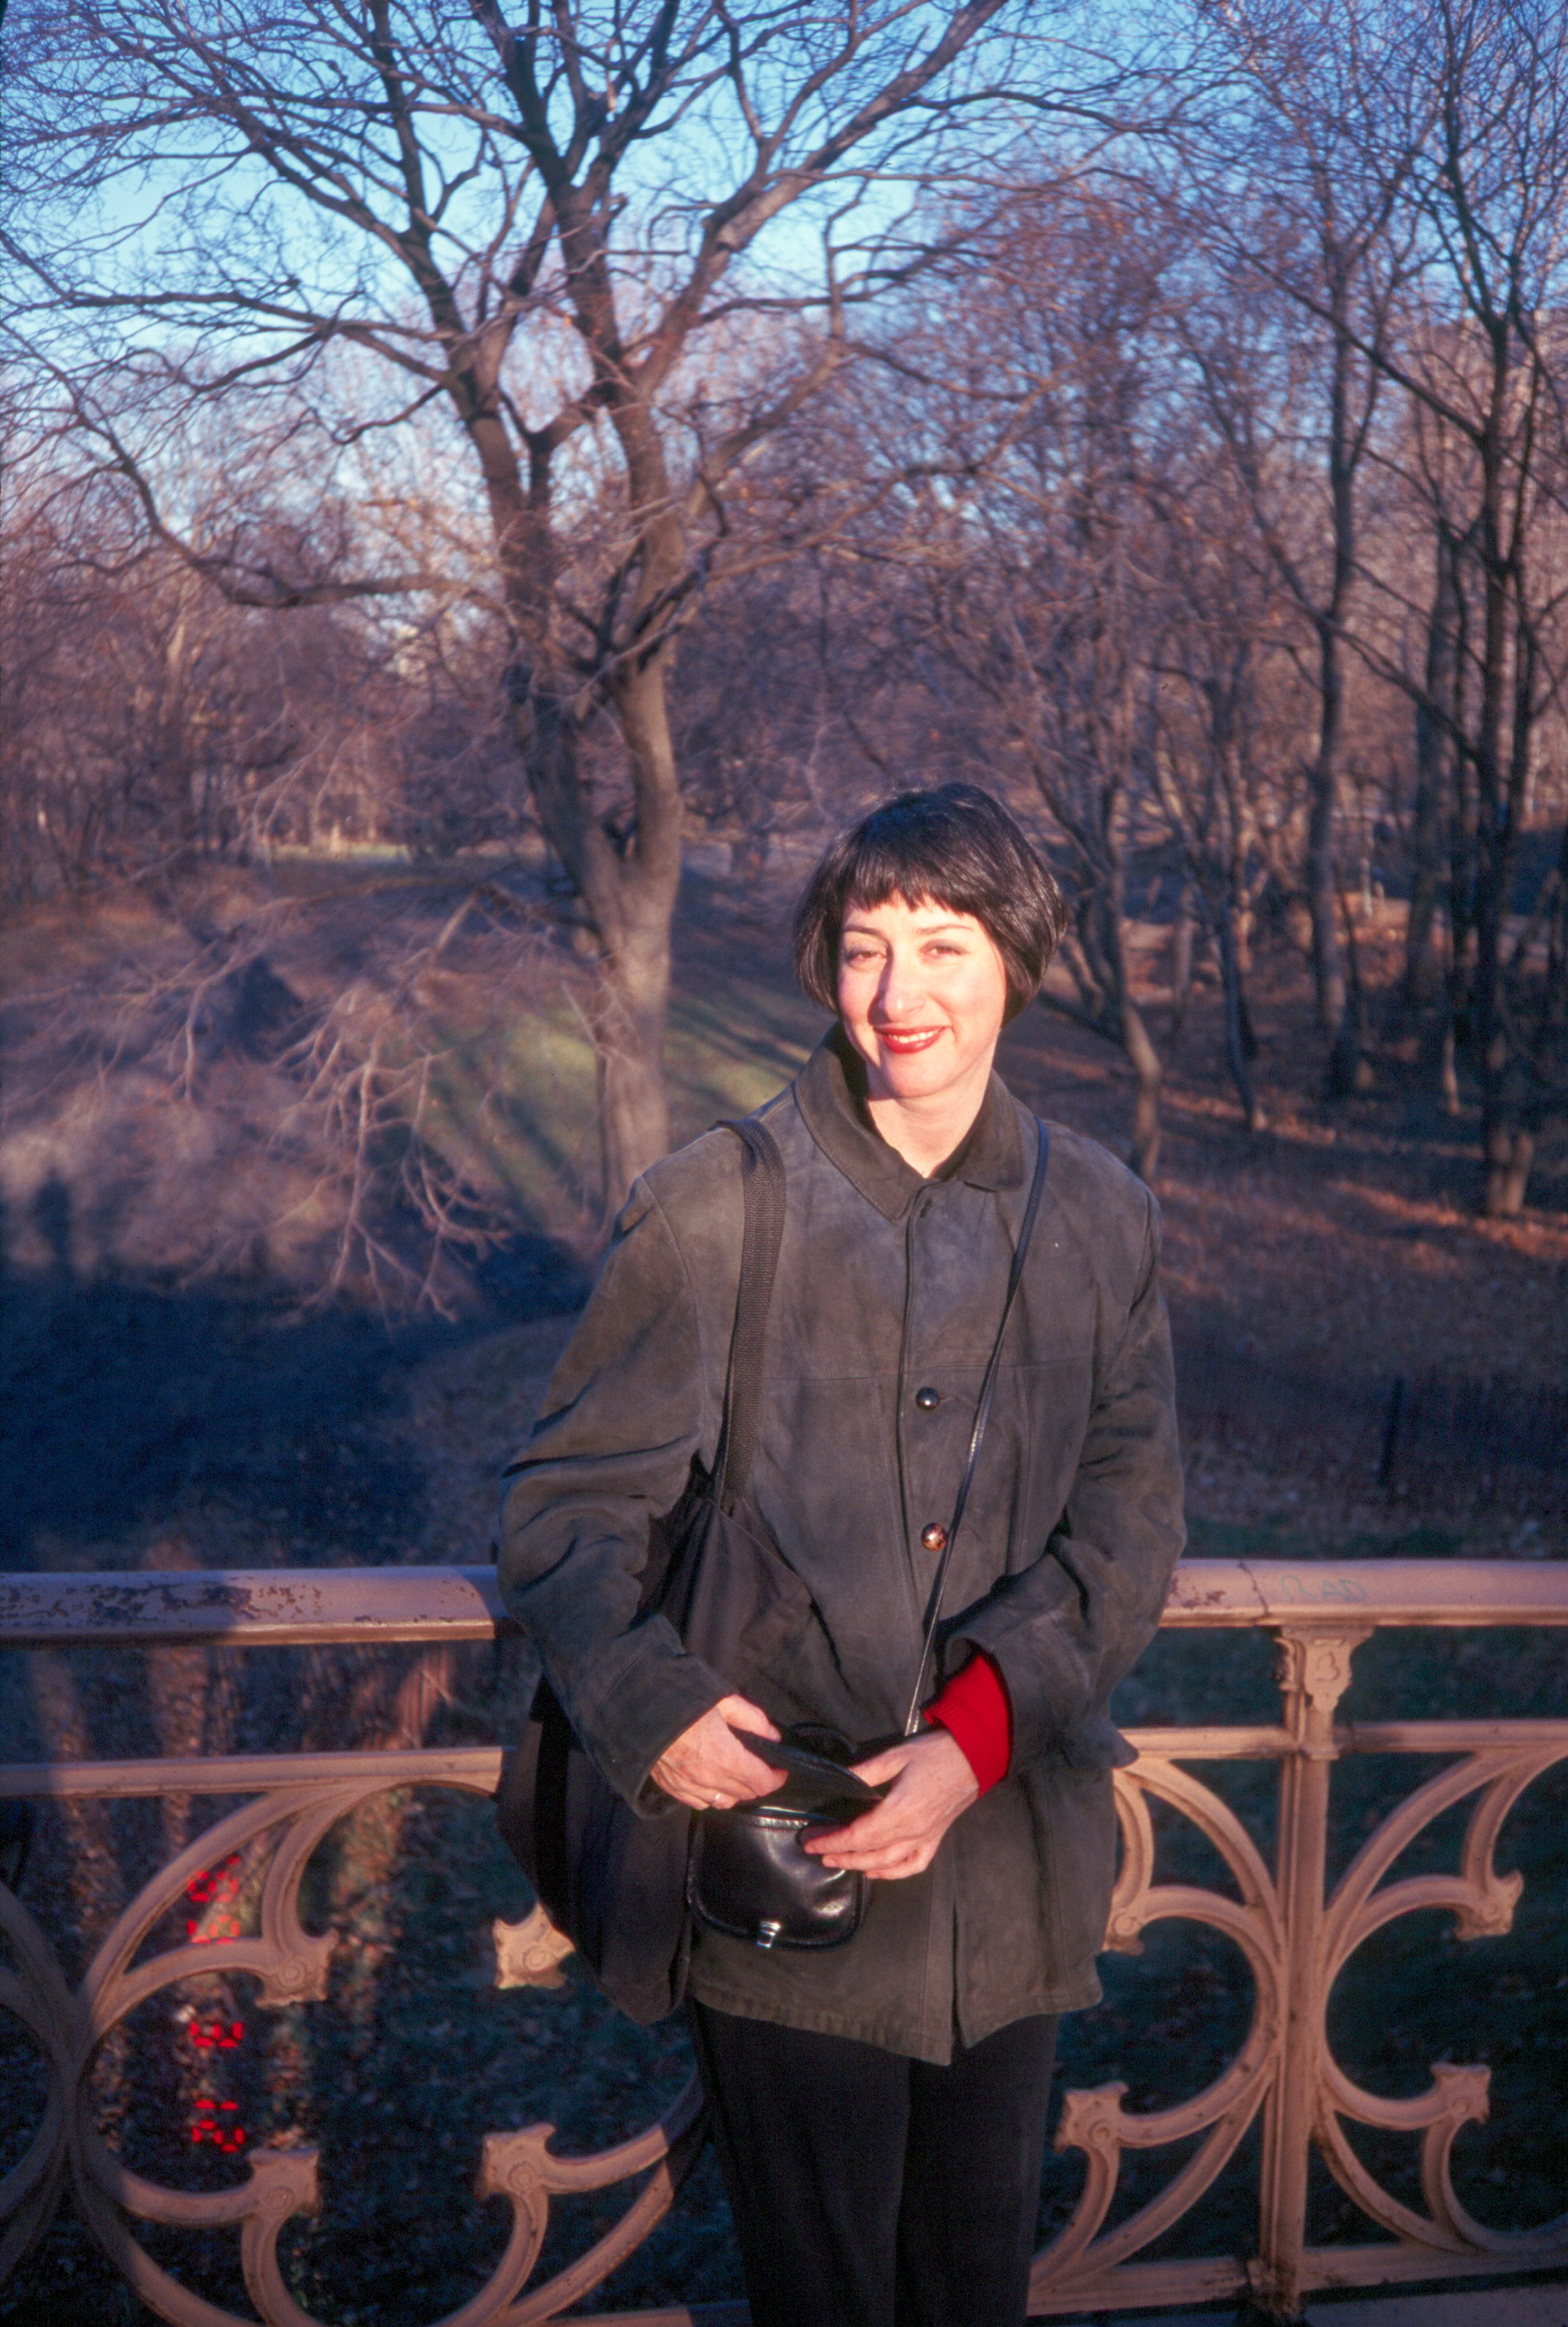
\includegraphics[width=\linewidth,height=\textheight,keepaspectratio]{/home/mkg/Dropbox/images/Heidi in Central Park.jpg}
    \captionlistentry[figure]{\url{\protect\detokenize{My wife Heidi, in Central Park, New York City, before we were married.}}}
\end{figure}

\KOMAoptions{pagesize}
\clearpage
\recalctypearea
\newpage
\noindent
Filename: None\\ 
Date taken: 2018:02:16 20:13:59\\ 
GPS longitude: (58.0, 23.0, 19.699)\\ 
GPS latitude: (34.0, 35.0, 41.0521)\\ 
Make: samsung\\ 
Model: SM-N950U\\ 
Focal length (35mm eq): 26\\ 
Exposure: 0.1\\ 
F stop: 1.7\\ 
ISO: 1250\\ 
Width: 4032\\ 
Height: 3024\\ 

\clearpage
\recalctypearea
\newpage
\noindent
\begin{figure}
    \includegraphics[width=\linewidth,height=\textheight,keepaspectratio]{/home/mkg/Dropbox/images/SM-950U/20180216_201359.jpg}
    \captionlistentry[figure]{\url{\protect\detokenize{Recoleta, Buenos Aires, Argentina.}}}
\end{figure}




\end{document}

